\documentclass[a4paper,UKenglish,cleveref, autoref, thm-restate, anonymous]{lipics-v2021}
%This is a template for producing LIPIcs articles. 
%See lipics-v2021-authors-guidelines.pdf for further information.
%for A4 paper format use option "a4paper", for US-letter use option "letterpaper"
%for british hyphenation rules use option "UKenglish", for american hyphenation rules use option "USenglish"
%for section-numbered lemmas etc., use "numberwithinsect"
%for enabling cleveref support, use "cleveref"
%for enabling autoref support, use "autoref"
%for anonymousing the authors (e.g. for double-blind review), add "anonymous"
%for enabling thm-restate support, use "thm-restate"
%for enabling a two-column layout for the author/affilation part (only applicable for > 6 authors), use "authorcolumns"
%for producing a PDF according the PDF/A standard, add "pdfa"

%\pdfoutput=1 %uncomment to ensure pdflatex processing (mandatatory e.g. to submit to arXiv)
%\hideLIPIcs  %uncomment to remove references to LIPIcs series (logo, DOI, ...), e.g. when preparing a pre-final version to be uploaded to arXiv or another public repository

%\graphicspath{{./graphics/}}%helpful if your graphic files are in another directory


\usepackage{amsmath}
%\let\proof\relax
%\let\endproof\relax

\sloppy


\usepackage{amsthm}
\usepackage{amssymb}
\usepackage{amsfonts}
\usepackage{mathrsfs}
\usepackage{wrapfig} %wrap the text around the picture


\usepackage{thmtools} 
\usepackage{thm-restate}

\usepackage{caption} %for subfigure - join multiple figures and add captions
%\usepackage{subcaption}
\usepackage{changepage} %inside figure we can put \begin{adjustwidth}{-1cm}{-1cm} \end{adjustwidth} and we can ignore the margins
\usepackage{mathtools} % write text [under]{over} arrow $\xrightarrow[\text{world}]{\text{hello}}$

\usepackage{graphicx}
\graphicspath{{Figures/}}

\usepackage{tikz}

\usetikzlibrary{arrows,decorations.pathmorphing,decorations.pathreplacing,backgrounds,positioning,fit,matrix}
\usetikzlibrary{shapes,calc,patterns,arrows.meta}
\tikzset{
	vert/.style={circle,inner sep=1.5,fill=white,draw,minimum size=.3cm},
	edge/.style={color=black, thick},
	diredge/.style={->,>={Stealth[width=8pt,length=8pt]},color=black, thick},
	timelabel/.style={fill=white,font=\footnotesize, text centered},
	wave/.style={decorate,decoration={coil,aspect=0}},
	dirwave/.style={->, >={Stealth[width=8pt,length=8pt]},decorate,decoration={coil,aspect=0}},
	diredge2/.style={->,>={Stealth[width=8pt,length=8pt]}}
}

%\usepackage{enumitem} %enumerate 
\usepackage{enumerate}
\usepackage{todonotes}
\newcommand{\todonkl}[2][]{\todo[color=red!100!green!33,#1]{NKL:\\ #2}} %todo note that starts with NKL:
\setlength{\marginparwidth}{3.7cm} %setting the length of todonote


\usepackage{comment}

\usepackage{algorithm}
\usepackage[noend]{algpseudocode}


%font encoding
\usepackage[T1]{fontenc}
\usepackage[utf8]{inputenc}
\usepackage{lmodern}

\usepackage{hyperref}

\crefname{claim}{Claim}{Claims}

%\usepackage{natbib}

\newcommand{\ie}{i.\,e.,\ }
\renewcommand{\st}{s.\,t.,\ }
\newcommand{\NP}{\textrm{NP}}
\newcommand{\APX}{\textrm{APX}}
\newcommand{\FPT}{\textrm{FPT}}
\newcommand{\XP}{\textrm{XP}}

\newcommand{\NN}{\mathbb{N}}
\newcommand{\ZZ}{\mathbb{Z}}
\newcommand{\RR}{\mathbb{R}}
\newcommand{\QQ}{\mathbb{Q}}


%%%%%%%%%%%%%%%%%%%%%%%%%%%%%%%% Defining a problem
%%%%%%%%%%%%%%%%%%\problemdef{NAME} {Input} {Output}
\usepackage{tabularx}
\newcommand{\problemdef}[3]{
	\begin{center}
		\begin{minipage}{0.95\textwidth}
			\noindent
			#1
			\vspace{5pt}\\
			\setlength{\tabcolsep}{3pt}
			\begin{tabularx}{\textwidth}{@{}lX@{}}
				\textbf{Input:}& #2 \\
				\textbf{Question:}& #3
			\end{tabularx}
		\end{minipage}
	\end{center}
}

\newcounter{guesscounter}


%%%%%%%%%%%%%%%%%%%%%%%%%%%%%%%%%% PROBLEMS NAMES
%% One label per edge, period Delta, exact realization
\newcommand{\deltaExactLong}{\textsc{Simple periodic Temporal Graph Realization}}
\newcommand{\deltaExact}{\textsc{Simple TGR}}

%% k labels per edge, period Delta, exact realization
\newcommand{\kDeltaExactLong}{\textsc{$(k,\Delta)$-periodic Exact Temporal Graph Realization}}
\newcommand{\kDeltaExact}{\textsc{$(k,\Delta)$-TGR}}

%% One label per edge, period Delta, upper-bounded realization
\newcommand{\kDeltaUpperBoundLong}{\textsc{Simple $\Delta$-periodic Upper-Bounded Temporal Graph Realization}}
%\newcommand{\deltaUpperBound}{}

%% k labels per edge, period Delta, lower-bound realization
\newcommand{\kDeltaLowerBoundLong}{\textsc{Simple $\Delta$-periodic Lower-Bounded Temporal Graph Realization}}


\bibliographystyle{plainurl}% the mandatory bibstyle
\usepackage{cite} %order citations by increasing number
\title{Temporal graph realization from fastest paths} %TODO Please add
%%%Realizing temporal graphs from fastest travel times

%\titlerunning{Dummy short title} %TODO optional, please use if title is longer than one line

\author{Nina Klobas}{Department of Computer Science, Durham University, UK}{nina.klobas@durham.ac.uk}{ https://orcid.org/0000-0002-8024-5782}{}

\author{George B. Mertzios}{Department of Computer Science, Durham University, UK}{george.mertzios@durham.ac.uk}{https://orcid.org/0000-0001-7182-585X}{Supported by the EPSRC grant EP/P020372/1.}

\author{Hendrik~Molter}{Department of Computer Science, Ben-Gurion~University~of~the~Negev, Beer-Sheva, Israel}{molterh@post.bgu.ac.il}{https://orcid.org/0000-0002-4590-798X}{Supported by the ISF, grant No.~1456/18, and the ERC, grant number 949707.}

\author{Paul G. Spirakis}{Department of Computer Science, University of Liverpool, UK}{p.spirakis@liverpool.ac.uk}{https://orcid.org/0000-0001-5396-3749}{Supported by the EPSRC grant EP/P02002X/1.}

\authorrunning{Nina Klobas, George B. Mertzios, Hendrik Molter, and Paul G. Spirakis} %TODO mandatory. First: Use abbreviated first/middle names. Second (only in severe cases): Use first author plus 'et al.'

\Copyright{Nina Klobas, George B. Mertzios, Hendrik Molter, and Paul G. Spirakis} %TODO mandatory, please use full first names. LIPIcs license is "CC-BY";  http://creativecommons.org/licenses/by/3.0/

\ccsdesc[500]{Theory of computation~Graph algorithms analysis}
\ccsdesc[500]{Mathematics of computing~Discrete mathematics}
%TODO mandatory: Please choose ACM 2012 classifications from https://dl.acm.org/ccs/ccs_flat.cfm 

\keywords{Temporal graph, periodic temporal labeling, fastest temporal path, graph realization, temporal connectivity.} %TODO mandatory; please add comma-separated list of keywords

\category{} %optional, e.g. invited paper

\relatedversion{} %optional, e.g. full version hosted on arXiv, HAL, or other respository/website
%\relatedversiondetails[linktext={opt. text shown instead of the URL}, cite=DBLP:books/mk/GrayR93]{Classification (e.g. Full Version, Extended Version, Previous Version}{URL to related version} %linktext and cite are optional

%\supplement{}%optional, e.g. related research data, source code, ... hosted on a repository like zenodo, figshare, GitHub, ...
%\supplementdetails[linktext={opt. text shown instead of the URL}, cite=DBLP:books/mk/GrayR93, subcategory={Description, Subcategory}, swhid={Software Heritage Identifier}]{General Classification (e.g. Software, Dataset, Model, ...)}{URL to related version} %linktext, cite, and subcategory are optional

%\funding{(Optional) general funding statement \dots}%optional, to capture a funding statement, which applies to all authors. Please enter author specific funding statements as fifth argument of the \author macro.

%\acknowledgements{I want to thank \dots}%optional

%\nolinenumbers %uncomment to disable line numbering



%Editor-only macros:: begin (do not touch as author)%%%%%%%%%%%%%%%%%%%%%%%%%%%%%%%%%%
\EventEditors{John Q. Open and Joan R. Access}
\EventNoEds{2}
\EventLongTitle{42nd Conference on Very Important Topics (CVIT 2016)}
\EventShortTitle{CVIT 2016}
\EventAcronym{CVIT}
\EventYear{2016}
\EventDate{December 24--27, 2016}
\EventLocation{Little Whinging, United Kingdom}
\EventLogo{}
\SeriesVolume{42}
\ArticleNo{23}
%%%%%%%%%%%%%%%%%%%%%%%%%%%%%%%%%%%%%%%%%%%%%%%%%%%%%%













\begin{document}
\maketitle

\begin{abstract}
In this paper we initiate the study of the \emph{temporal graph realization} problem with respect to the fastest path durations among its vertices, 
while we focus on periodic temporal graphs. 
Given an $n \times n$ matrix $D$ and a $\Delta \in \mathbb{N}$, the goal is to construct a $\Delta$-periodic temporal graph with $n$ vertices 
such that the duration of a \emph{fastest path} from $v_i$ to $v_j$ is equal to $D_{i,j}$, or to decide that such a temporal graph does not exist. 
The variations of the problem on static graphs has been well studied and understood since the 1960's (e.g.\ [Erd\H{o}s and Gallai, 1960], [Hakimi and Yau, 1965]).
% , and this area of research remains active until nowadays. 

As it turns out, the periodic temporal graph realization problem has a very different computational complexity behavior than its static (\ie non-temporal) counterpart. 
First we show that the problem is NP-hard in general, but polynomial-time solvable if the so-called underlying graph is a tree.
Building upon those results, we investigate its parameterized computational complexity with respect to structural parameters of the underlying static graph which measure the ``tree-likeness''. We prove a tight classification between such parameters that allow fixed-parameter tractability (FPT) 
and those which imply W[1]-hardness. 
We show that our problem is W[1]-hard when parameterized by the \emph{feedback vertex number} (and therefore also any smaller parameter such as \emph{treewidth}, \emph{degeneracy}, and \emph{cliquewidth}) of the underlying graph, while we show that it is in FPT when parameterized by the \emph{feedback edge number} (and therefore also any larger parameter such as \emph{maximum leaf number}) of the underlying graph. 





\vspace{0,2cm}
\noindent \textbf{Due to lack of space, the full paper with all proofs is attached in a 
	clearly marked Appendix to be read at the discretion of the Program Committee.}
\end{abstract}

\clearpage

\section{Introduction}\label{intro-sec}

The (static) \emph{graph realization} problem with respect to a graph property $\mathcal{P}$ is to find a graph that satisfies property $\mathcal{P}$, or to decide that no such graph exists. 
The motivation for graph realization problems stems both from ``verification'' and from network design applications in engineering. 
In \emph{verification} applications, given the outcomes of some experimental measurements (resp.~some computations) on a network, 
the aim is to (re)construct an input network which complies with them. 
If such a reconstruction is not possible, this proves that the measurements are incorrect or implausible (resp.~that the algorithm which made the computations is incorrectly implemented). 
One example of a graph realization (or reconstruction) problem is the recognition of probe interval graphs, in the context of the physical mapping of DNA, see~\cite{McMorris98,McConnellS02} and~\cite[Chapter 4]{GolumbicTrenk04}.
In \emph{network design} applications, the goal is to design network topologies having a desired property~\cite{augustine2022distributed,grotschel1995design}.
Analyzing the computational complexity of the graph realization problems for various natural and fundamental graph properties $\mathcal{P}$ requires a deep understanding of these properties.
Among the most studied such parameters for graph realization 
are constraints on the distances between vertices~\cite{barNoy2022GraphRealization,barNoy2021composed,hakimi1965distance,chung2001distance,bixby1988almost,culberson1989fast}, 
on the vertex degrees~\cite{GolovachM17,gomory1961multi,hakimi1962realizability,Bar-NoyCPR20,erdos1960graphs}, 
%%%%barNoy2021selected,cai2000solution
on the eccentricities~\cite{barNoy2020efficiently,hell2009linear,behzad1976eccentric,lesniak1975eccentric}, and on connectivity~\cite{fulkerson1960zero,frank1992augmenting,chen1966realization,frank1994connectivity,frank1970connectivity,gomory1961multi}, among others. 


In the simplest version of a (static) graph realization problem with respect to vertex distances, 
we are given a symmetric $n \times n$ matrix $D$ and we are looking for an $n$-vertex undirected and unweighted graph $G$ such that $D_{i,j}$ equals the distance between vertices $v_i$ and $v_j$ in~$G$. This problem can be trivially solved in polynomial time in two steps~\cite{hakimi1965distance}: First, we build the graph $G=(V,E)$ such that $v_i v_j \in E$ if and only if $D_{i,j}=1$. Second, from this graph $G$ we compute the matrix $D_G$ which captures the shortest distances for all pairs of vertices. If $D_G = D$ then $G$ is the desired graph, otherwise there is no graph having $D$ as its distance matrix. 
Non-trivial variations of this problem have been extensively studied, such as for weighted graphs~\cite{hakimi1965distance,Patrinos-Hakimi-72}, as well as for cases where the realizing graph has to belong to a specific graph family~\cite{hakimi1965distance, barNoy2021composed}. Other variations of the problem include the cases where every entry of the input matrix $D$ may contain a range of consecutive permissible values~\cite{barNoy2021composed,Rubei16,Tamura93}, or even an arbitrary set of acceptable values~\cite{barNoy2022GraphRealization} for the distance between the corresponding two vertices. 

In this paper we make the first attempt to understand the complexity of the graph realization problem with respect to vertex distances in the context of \emph{temporal graphs}, \ie of graphs whose \emph{topology changes over time}. 

\begin{definition}[temporal graph~\cite{KKK00}]
\label{temp-graph-def} A \emph{temporal graph} is a pair $(G,\lambda)$,
where $G=(V,E)$ is an underlying (static) graph and $\lambda :E\rightarrow 2^\mathbb{N}$ is a \emph{time-labeling} function which assigns to every edge of $G$ a set of discrete time-labels.
\end{definition}

Here, whenever $t \in \lambda(e)$, we say that the edge $e$ is \emph{active} or \emph{available} at time $t$. In the context of temporal graphs, where the notion of vertex adjacency is time-dependent, the notions of path and distance also need to be redefined. The most natural temporal analogue of a path is that of a \emph{temporal} (or \emph{time-dependent}) path, which is motivated by the fact that, due to
causality, entities and information in temporal graphs can ``flow'' only along sequences of
edges whose time-labels are strictly increasing.

\begin{definition}[fastest temporal path] \label{def:temporalPath+Duration}
Let $(G,\lambda)$ be a temporal graph. A \emph{temporal path} 
in $(G,\lambda)$ is a sequence $(e_1,t_1),(e_2,t_2),\ldots,(e_k,t_k)$, 
where $P=(e_1,\ldots,e_k)$ is a path in the underlying static graph $G$, 
%(we usually say that $P$ is the underlying path of $(P,\lambda)$), 
$t_i\in \lambda(e_i)$ for every $i=1,\ldots,k$, and $t_1<t_2<\ldots<t_k$. 
The \emph{duration} of this temporal path %$(P,\lambda)$ from $u$ to $v$ 
is $t_k - t_1 + 1$.
A \emph{fastest} temporal path from a vertex $u$ to a vertex $v$ in $(G,\lambda)$ is a temporal path from $u$ to $v$ with the smallest duration.
The \emph{duration} of the fastest temporal path from $u$ to $v$ is denoted by $d(u,v)$.
\end{definition}

%Other temporal analogues of a shortest path are temporal paths with the smallest total number of edges (\emph{shortest} temporal path), or the smallest earliest arrival time (\emph{foremost} temporal path), respectively. 







In this paper we consider \emph{periodic} temporal graphs, \ie temporal graphs in which the temporal availability of each edge of the underlying graph is periodic. 
Many natural and technological systems exhibit a periodic temporal behavior. For example, in railway networks an edge is present at a time step $t$ if and
only if a train is scheduled to run on the respective rail segment at time $t$~\cite{Arrighi2023Multi}. 
Similarly, a satellite, which makes pre-determined periodic movements, can establish a communication link (\ie a temporal edge) with another satellite whenever they are sufficiently close to each other; the existence of these communication links is also periodic. 
In a railway (resp.~satellite) network, a fastest temporal path from $u$ to $v$ represents the fastest railway connection between two stations 
(resp.~the quickest communication delay between two moving satellites). 
Furthermore, periodicity appears also in (the otherwise quite complex) social networks which describe the dynamics of people meeting~\cite{snapnets,sapiezynski2015tracking}, as every person individually follows mostly a daily routine~\cite{Arrighi2023Multi}. 


Although periodic temporal graphs have already been studied 
(see~\cite[Class 8]{casteigts2012time} and~\cite{Arrighi2023Multi,ErlebachS20,morawietz2021timecop,morawietz2020timecop}), 
we make here the first attempt to understand the complexity of a graph realization problem in the context of temporal graphs. 
Therefore, we focus in this paper on the most fundamental case, where all edges have the same period $\Delta$ 
(while in the more general case, each edge $e$ in the underlying graph has a period $\Delta_e$).
As it turns out, the periodic temporal graph realization problem with respect to a given $n \times n$ matrix $D$ of the fastest duration times has a very different computational complexity behavior than the classic graph realization problem with respect to shortest path distances in static graphs. 








Formally, let $G=(V,E)$ and $\Delta\in \mathbb{N}$, and let $\lambda: E \rightarrow \{1,2,\ldots,\Delta\}$ be an edge-labeling function that assigns to every edge of $G$ exactly one of the labels from $\{1,\ldots,\Delta\}$. 
Then we denote by $(G,\lambda,\Delta)$ the \emph{$\Delta$-periodic temporal graph} $(G,L)$, where for every edge $e\in E$ we have $L(e)=\{i\Delta + x : i\geq 0, x\in \lambda(e)\}$. 
In this case we call $\lambda$ a \emph{$\Delta$-periodic labeling} of~$G$; see \cref{fig:periodic-example} for an illustration. 
When it is clear from the context, we drop $\Delta$ form the notation and 
we denote the ($\Delta$-periodic) temporal graph by $(G,\lambda)$.
Given a duration matrix~$D$, it is easy to observe that, similarly to the static case, if $D_{i,j}=1$ then $v_i$ and $v_j$ must be connected by an edge. We call the graph defined by these edges the \emph{underlying graph} of $D$.



\subparagraph{Our contribution.}
%In this work, 
We initiate the study of naturally motivated graph realization problems in the temporal setting. 
Our target is not to model unreliable communication, but instead to \emph{verify} that particular measurements regarding fastest temporal paths in a periodic temporal graph are plausible (\ie ``realizable''). 
To this end, we introduce and investigate the following problem, capturing the setting described above:
	
	
\problemdef{\deltaExactLong\ (\deltaExact)}
{An $n \times n$ matrix $D$, a positive integer $\Delta$.}
{Does there exist a graph $G=(V,E)$ with vertices $\{v_1,\ldots,v_{n}\}$ 
and a $\Delta$-periodic labeling $\lambda: E \rightarrow \{1,2,\ldots,\Delta\}$ such that, 
for every $i,j$, the duration of the fastest temporal path from $v_i$ to $v_j$ in the $\Delta$-periodic temporal graph $(G,\lambda,\Delta)$ is $D_{i,j}$?}


\begin{figure}[t]
    \centering
	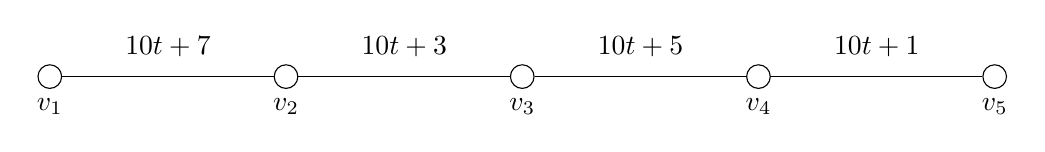
\begin{tikzpicture}[xscale=1.5]
		%%%S_uv
		\node[vert,label=below:$v_1$] (1) at (1,0) {};
		\node[vert,label=below:$v_2$] (2) at (3,0) {};
		\node[vert,label=below:$v_3$] (3) at (5,0) {};
		\node[vert,label=below:$v_4$] (4) at (7,0) {};
		\node[vert,label=below:$v_5$] (5) at (9,0) {};
		\draw (1) -- node[label=above:$10t+7$] {} (2) -- node[label=above:$10t+3$] {}  (3) -- node[label=above:$10t+5$] {} (4) -- node[label=above:$10t+1$] {} (5);	
	\end{tikzpicture}
	\caption{An example of a $\Delta$-periodic temporal graph $(G,\lambda,\Delta)$, where $\Delta = 10$ and the 10-periodic labeling $\lambda: E \rightarrow \{1,2,\ldots,10\}$ is as follows: $\lambda(v_1 v_2)=7$, $\lambda(v_2 v_3)=3$, $\lambda(v_3 v_4)=5$, and $\lambda(v_4 v_5)=1$. 
    Here, the fastest temporal path from $u$ to $v$ traverses the first edge $v_1v_2$ at time $7$, second edge $v_2v_3$ a time $13$, third edge $v_3v_4$ at time $15$ and the last edge $v_4v_5$ at time $21$.
    This results in the total duration of $15$ for the fastest temporal path from $v_1$ to $v_5$.
	\label{fig:periodic-example}}
\end{figure}

We focus on exact algorithms. We start by showing NP-hardness of the problem (\cref{thm:NPhardness}), even if $\Delta$ is a small constant. To establish a baseline for tractability, we show that \deltaExact\ is polynomial-time solvable if the underlying graph is a tree (\cref{thm:deltaExact-PolyTimeTrees}).

Building upon these initial results, we explore the possibilities to generalize our polynomial-time algorithm using the \emph{distance-from-triviality} parameterization paradigm~\cite{FJR13,GHN04}. That is, we investigate the parameterized computational complexity of \deltaExact\ with respect to structural parameters of the underlying graph that measure its ``tree-likeness''.

We obtain the following results. We show that \deltaExact\ is W[1]-hard when parameterized by the \emph{feedback vertex number} of the underlying graph (\cref{thm:W1wrtFVS}). 
To this end, we first give a reduction from \textsc{Multicolored Clique} parameterized by the number of colors~\cite{fellows2009multipleinterval} to a variant of \deltaExact\ where the period $\Delta$ is infinite, that is, when the labeling is non-periodic. We use a special gadget (the ``infinity'' gadget) which allows us to transfer the result to a finite period $\Delta$. The latter construction is independent from the particular reduction we use, and can hence be treated as a reduction from the non-periodic to the periodic setting.
Note that our parameterized hardness result with respect to the feedback vertex number 
also implies W[1]-hardness for any smaller parameter, such as \emph{treewidth}, \emph{degeneracy}, \emph{cliquewidth}, 
\emph{distance to chordal graphs}, and \emph{distance to outerplanar graphs}.


We complement this hardness result by showing that \deltaExact\ is fixed-parameter tractable (FPT) with respect to the \emph{feedback edge number} $k$ of the underlying graph (\cref{thm:FPTwrtFES}). 
This result also implies an FPT algorithm for any larger parameter, such as the \emph{maximum leaf number}. 
A similar phenomenon of getting W[1]-hardness with respect to the feedback vertex number, while getting an FPT algorithm with respect to the feedback edge number, has been observed only in a few other temporal graph problems related to the connectivity between two vertices~\cite{casteigts2021finding,FMNR22a,EMM22}.

Our FPT algorithm works as follows on a high level. 
First we distinguish $O(k^2)$ vertices which we call ``important vertices''. 
Then, we guess the fastest temporal paths for each pair of these important vertices; as we prove, the number of choices we have for all these guesses is upper bounded by a function of~$k$. 
Then we also need to make several further guesses (again using a bounded number of choices), which altogether leads us to specify a small (\ie bounded by a function of $k$) number of different configurations for the fastest paths between \emph{all pairs} of vertices. For each of these configurations, we must then make sure that the labels of our solution will not allow any other temporal path from a vertex $v_i$ to a vertex $v_j$ have a \emph{strictly smaller} duration than~$D_{i,j}$.
This naturally leads us to build one Integer Linear Program (ILP) for each of these configurations. We manage to formulate all these ILPs by having a number of variables that is upper-bounded by a function of $k$. Finally we use Lenstra's Theorem~\cite{Lenstra1983Integer} to solve each of these ILPs in FPT time. At the end, our initial instance is a \textsc{Yes}-instance if and only if at least one of these ILPs is feasible.




The above results provide a fairly complete picture of the parameterized computational complexity of \deltaExact\ with respect to structural parameters of the underlying graph which measure ``tree-likeness''. To obtain our results, we prove several properties of fastest temporal paths, which may be of independent interest. 
Due to space constraints, proofs of results marked with $\star$ are (partially) deferred to the Appendix.


\subparagraph{Related work.} Graph realization problems on static graphs have been studied since the 1960s. We provide an overview of the literature in the introduction. 
To the best of our knowledge, we are the first to consider graph realization problems in the temporal setting. However, many other connectivity-related problems have been studied in the temporal setting~\cite{Mertzios-transitivity21,Akrida-explorer-21,enright2021deleting,MolterRZ21,klobas2023interference,deligkas2022optimizing,erlebach2021temporal,Flu+19a,Zsc+19,CasteigtsCS22,FuchsleMNR22}, most of which are much more complex and computationally harder than their non-temporal counterparts, and some of which do not even have a non-temporal counterpart.

There are some problem settings that share similarities with ours, which we discuss now in more detail.

Several problems have been studied where the goal is to assign labels to (sets of) edges of a given static graph in order to achieve certain connectivity-related properties~\cite{KlobasMMS22,MertziosMS19,akrida2017complexity,enright2021assigning}. The main difference to our problem setting is that in the mentioned works, the input is a graph and the sought labeling is not periodic. Furthermore, the investigated properties are temporal connectivity among all vertices~\cite{KlobasMMS22,MertziosMS19,akrida2017complexity}, temporal connectivity among a subset of vertices~\cite{KlobasMMS22}, or reducing reachability among the vertices~\cite{enright2021assigning}. In all these cases, the duration of the temporal paths has not been considered.


%work on the temporal cops and robber game~\cite{morawietz2021timecop,morawietz2020timecop,ErlebachS20}. The question here is (in its basic case) whether a certain number of cops are able to catch a robber, if everybody can move along one edge at every time step and the robber is considered caught if it occupies the same vertex as a cop at the same time. Several other works on periodic temporal graphs were mentioned in the introduction.


Finally, there are many models for dynamic networks in the context of distributed computing~\cite{Kuhn2011Dynamic}. 
These models have some similarity to temporal graphs, in the sense that in both cases the edges appear and disappear over time. 
However, there are notable differences. For example, one important assumption in the distributed setting 
can be that the edge changes are adversarial or random (while obeying some constraints such as connectivity), 
and therefore they are not necessarily known in advance~\cite{Kuhn2011Dynamic}. 




\subparagraph{Preliminaries and notation.}
We already introduced the most central notion and concepts. There are some additional definitions we need, to present our proofs and results which we give in the following. 

An interval in $\mathbb N$ from $a$ to $b$ is denoted by $[a,b] = \{ i\in \mathbb N  :  a \leq i \leq b\}$; similarly, $[a] = [1,a]$.
An undirected graph~$G=(V,E)$ consists of a set~$V$ of vertices 
and a set~$E \subseteq V \times V$ of edges.
For a graph~$G$, we also denote by~$V(G)$ and~$E(G)$ the vertex and edge set of~$G$, respectively.
We denote an edge $e \in E$ between vertices $u,v \in V$ as a set $e=\{u,v\}$.
For the sake of simplicity of the representation, an edge $e$ is sometimes also denoted by $uv$. 
A path~$P$ in $G$ is a subgraph of $G$ with vertex set~$V(P)=\{v_1,\dots,v_k\}$ and edge set~$E(P)=\{\{v_i,v_{i+1}\} :  1\leq i<k\}$
(we often represent path~$P$ by the tuple~$(v_1,v_2,\dots,v_k)$).

Let $v_1,v_2,\ldots,v_n$ be the $n$ vertices of the graph $G$. 
For simplicity of the presentation (and with a slight abuse of notation) we refer during the paper to the entry $D_{i,j}$ of the matrix $D$ as $D_{a,b}$, where $a=v_i$ and $b=v_j$. 
That is, we put as indices of the matrix $D$ the corresponding vertices of $G$ whenever it is clear from the context. 


Let $P=(u=v_1, v_2, \dots, v_p=v)$ be a path from $u$ to $v$ in $G$. 
Recall that, in our paper, every edge has exactly one time label in every period of $\Delta$ consecutive time steps. 
Therefore, as we are only interested in the fastest duration of temporal paths, 
many times we refer to $(P,\lambda,\Delta)$ as any of the temporal paths from $u=v_1$ to $v=v_p$ along the edges of $P$, which starts at the edge $v_1 v_2$ at time $\lambda(v_1 v_2) + c \Delta$, for some $c\in \mathbb{N}$, and then sequentially visits the rest of the edges of $P$ as early as possible. 
We denote by $d(P,\lambda,\Delta)$, or simply by $d(P,\lambda)$ when $\Delta$ is clear from the context, the duration of any of the temporal paths $(P,\lambda,\Delta)$; note that they all have the same duration. 
Many times we also refer to a path $P=(u=v_1, v_2, \dots, v_p=v)$ from $u$ to $v$ in $G$,
as a temporal path in $(G,\lambda,\Delta)$,
where we actually mean that $(P,\lambda,\Delta)$ is a temporal path with $P$ as its underlying (static) path.


We remark that a fastest path between two vertices in a temporal graph can be computed in polynomial time~\cite{xuan_computing_2003,Wu2016Efficient}.
%Wu et~al.~\cite{Wu2016Efficient} provide an algorithm that computes the duration of the fastest temporal path from a source vertex $v$, in a temporal graph $(G,\lambda)$, to all other vertices,
%that runs in polynomial-time.
Hence, given a $\Delta$-periodic temporal graph $(G,\lambda,\Delta)$, we can compute in polynomial-time  the matrix $D$
which consists of durations of fastest temporal paths among all pairs of vertices in $(G,\lambda,\Delta)$.

\begin{comment}
Let $(G,\lambda)$ be a temporal graph with  $n = |V(G)|$ and  $m=|E(G)|$.
Let $v \in V(G)$ be an arbitrary vertex of $G$, denote with $deg_{max}$ the maximum degree of all vertices in $V(G)$ and let $S_v$ be the set of time edges in $(G,\lambda)$, incident to $v$, \ie $S_v = \{(uv, \lambda(uv)) | uv \in E(G)\}$.
In their work Wu et~al.~\cite{Wu2016Efficient} provide an algorithm that computes the duration of the fastest temporal path from a source vertex $v$ to all other vertices in $G$ in
$O(n + m \log c)$ time, where $c = \min \{|S_v|, deg_{max}\}$.
From this result, we can deduce the following. 
\begin{lemma} \label{lemma:calculatingD}
Let $(G, \lambda, \Delta)$ be a $\Delta$-periodic temporal graph, where $\lambda$ assigns exactly $k$ labels to every edge of $G$. 
Denote with $deg_{max}$ the maximum degree of vertices in $G$, let $deg(v_i)$ be the degree of vertex $v_i \in V(G)$,
and let $c_{v_i} = \min \{ k \cdot deg(v_i), deg_{max}\}$.\\
To calculate the durations of all fastest temporal paths from a fixed vertex $v \in V(G)$ to all other vertices, it takes $O(n + m \log c_v)$ time. \\
To calculate the durations of the fastest temporal paths among all pairs of vertices we then need $O(n^2 + m \sum_{v \in V(G)} \log c_v)$ time.
\end{lemma}

Observe that $O(n + m \log c_v) = O(n + m \log deg_{max}) = O(n + m \log n) = O(n^2 \log n)$ and similarly
$O(n^2 + m \sum_{v \in V(G)} \log c_v) = O(n^2 + mn \log deg_{max}) = O(n + mn \log n) = O(n^3 \log n)$.
Since an instance $I$ of \kDeltaExact\ problem is an $n \times n$ matrix $D$, the running time of calculating one row of $D$ (\ie the fastest temporal paths from a single vertex to all others) takes $O(|I|\log \sqrt{|I|})$-time and calculating the whole matrix $D$ (\ie the fastest temporal paths among all pairs of vertices) takes $O(|I|^{3/2} \log \sqrt{|I|})$ time.
Therefore, from now on we say that calculating (a row of) $D$ takes polynomial time.
\end{comment}
%\section{Results}



\section{Hardness results for \deltaExact}  
In this section we present our main computational hardness results.  
We first show that \deltaExact\ is NP-hard even for constant $\Delta$. 
%Then we investigate the parameterized computational hardness of \deltaExact\ with respect to structural parameters of the underlying graph. We show that \deltaExact\ is W[1]-hard when parameterized by the feedback vertex number of the underlying graph.

%\subparagraph{NP-hardness of \deltaExact.}\label{sec:nphardness}
%We prove that in general it is NP-hard to determine a $\Delta$-periodic temporal graph $(G,\lambda)$ respecting a duration matrix $D$,
%even if $\Delta$ is a small constant.

\begin{theorem}[$\star$]\label{thm:NPhardness}
	\deltaExact\ is \NP-hard for all $\Delta \geq 3$.
\end{theorem}

\begin{comment}

\begin{proof}
	We present a polynomial-time reduction from the NP-hard problem NAE 3-SAT~\cite{Schaefer1978complexity}. Here we are given a formula $\phi$ that is a conjunction of so-called NAE (not-all-equal) clauses, where each clause contains exactly 3 literals (with three distinct variables).
    A NAE clause evaluates to \textsc{true} if and only if not all of its literals are equal, that is, at least one literal evaluates to \textsc{true} and at least one literal evaluates to \textsc{false}.
    We are asked whether $\phi$ admits a satisfying assignment. 

    
    Given an instance $\phi$ of NAE 3-SAT, we construct an instance $(D,\Delta)$ of \deltaExact\ as follows.

 We start by describing the vertex set of the underlying graph $G$ of $D$.
\begin{itemize}
\item For each variable $x_i$ in $\phi$, we create three variable vertices $x_i, x_i^T, x_i^F$.
\item For each clause $c$ in $\phi$, we create one clause vertex $c$.
\item We add one additional super vertex $v$.
\end{itemize}
Next, we describe the edge set of $G$.
\begin{itemize}
\item For each variable $x_i$ in $\phi$ we add the following five edges: 
$x_i x_i^T, x_i x_i^F, x_i^T x_i^F, x_i^T v$ and $ x_i^Fv$.
\item For each pair of variables $x_i,x_j$ in $\phi$ with $i \neq j$ we add the following four edges: 
$x_i^T x_j^T, x_i^Tx_j^F, x_i^Fx_j^T$ and $x_i^Fx_j^F$.
\item For each clause $c$ in $\phi$ we add one edge for each literal. Let $x_i$ appear in $c$. If $x_i$ appears non-negated in $c$ we add edge $c x_i^T$. 
If $x_i$ appears negated in $c$ we add edge $c x_i^F$.
\end{itemize}
This finishes the construction of $G$.
For an illustration see~\cref{fig:NP-example}.

%
\begin{figure}[htb]
	\noindent
	\makebox[\textwidth]{
		\centering
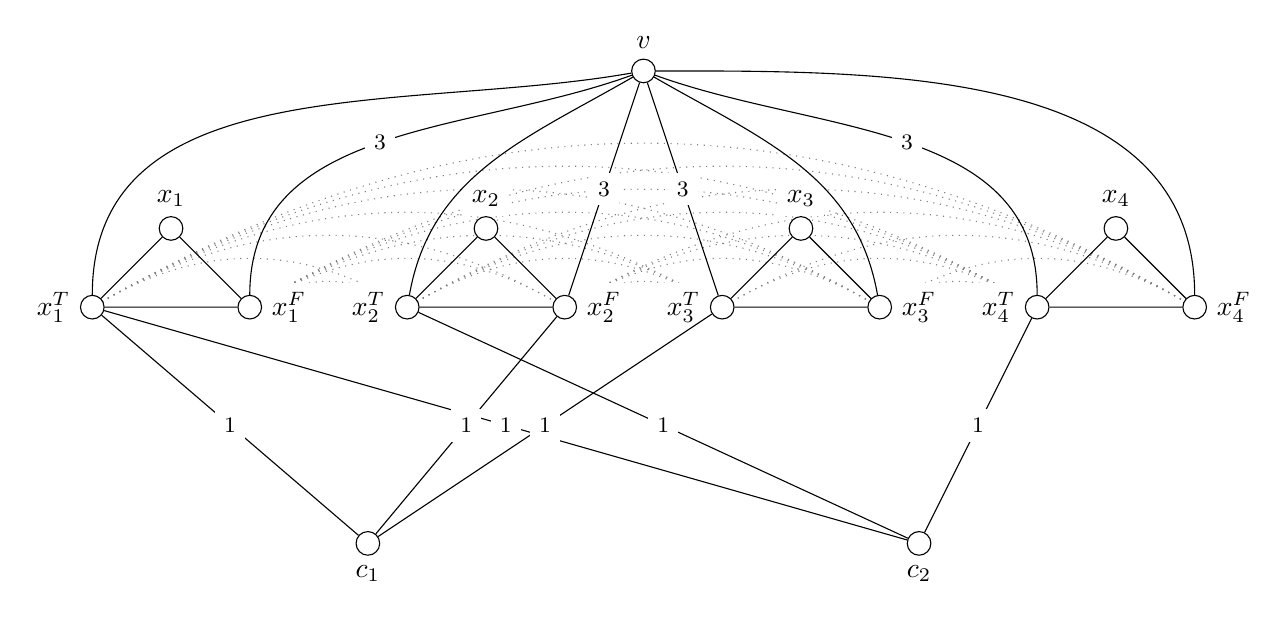
\begin{tikzpicture}%[xscale=2]

	%%Variable X1
	\node (x1t) at (1,0) {};
	\node (x1f) at (3,0) {};
	
	%%Variable X2
	\node (x2t) at (5,0) {};
	\node (x2f) at (7,0) {};
	
	%%Variable x3
	\node (x3t) at (9,0) {};
	\node (x3f) at (11,0) {};
	
	%%Variable x4
	\node (x4t) at (13,0) {};
	\node (x4f) at (15,0) {};

	%% edges among xt, xf vertices
	%x1 to all
	\draw [dotted,gray] (x1t) [out=30,in=150] to (x2t);
	\draw [dotted,gray] (x1t) [out=30,in=150] to (x3t);
	\draw [dotted,gray] (x1t) [out=30,in=150] to (x4t);
	\draw [dotted,gray] (x1t) [out=30,in=150] to (x2f);
	\draw [dotted,gray] (x1t) [out=30,in=150] to (x3f);
	\draw [dotted,gray] (x1t) [out=30,in=150] to (x4f);
	
	\draw [dotted,gray] (x1f) [out=30,in=150] to (x2t);
	\draw [dotted,gray] (x1f) [out=30,in=150] to (x3t);
	\draw [dotted,gray] (x1f) [out=30,in=150] to (x4t);
	\draw [dotted,gray] (x1f) [out=30,in=150] to (x2f);
	\draw [dotted,gray] (x1f) [out=30,in=150] to (x3f);
	\draw [dotted,gray] (x1f) [out=30,in=150] to (x4f);
	%x2 to all
	\draw [dotted,gray] (x2t) [out=30,in=150] to (x3t);
	\draw [dotted,gray] (x2t) [out=30,in=150] to (x4t);
	\draw [dotted,gray] (x2t) [out=30,in=150] to (x3f);
	\draw [dotted,gray] (x2t) [out=30,in=150] to (x4f);
	
	\draw [dotted,gray] (x2f) [out=30,in=150] to (x3t);
	\draw [dotted,gray] (x2f) [out=30,in=150] to (x4t);
	\draw [dotted,gray] (x2f) [out=30,in=150] to (x3f);
	\draw [dotted,gray] (x2f) [out=30,in=150] to (x4f);
	%x3 to all
	\draw [dotted,gray] (x3t) [out=30,in=150] to (x4t);
	\draw [dotted,gray] (x3t) [out=30,in=150] to (x4f);
	
	\draw [dotted,gray] (x3f) [out=30,in=150] to (x4t);
	\draw [dotted,gray] (x3f) [out=30,in=150] to (x4f);

	%%Variable X1
	\node[vert,label=left:$x_1^T$] (x1t) at (1,0) {};
	\node[vert,label={[fill=white]right:$x_1^F$}] (x1f) at (3,0) {};
	\node[vert,label=above:$x_1$] (x1) at (2,1) {};
	\draw (x1t) -- (x1f) -- (x1) -- (x1t);
	
	%%Variable X2
	\node[vert,label={[fill=white]left:$x_2^T$}] (x2t) at (5,0) {};
	\node[vert,label={[fill=white]right:$x_2^F$}] (x2f) at (7,0) {};
	\node[vert,label={[fill=white]above:$x_2$}] (x2) at (6,1) {};
	\draw (x2t) -- (x2f) -- (x2) -- (x2t);
	
	%%Variable x3
	\node[vert,label={[fill=white]left:$x_3^T$}] (x3t) at (9,0) {};
	\node[vert,label={[fill=white]right:$x_3^F$}] (x3f) at (11,0) {};
	\node[vert,label={[fill=white]above:$x_3$}] (x3) at (10,1) {};
	\draw (x3t) -- (x3f) -- (x3) -- (x3t);
	
	%%Variable x4
	\node[vert,label={[fill=white]left:$x_4^T$}] (x4t) at (13,0) {};
	\node[vert,label=right:$x_4^F$] (x4f) at (15,0) {};
	\node[vert,label=above:$x_4$] (x4) at (14,1) {};
	\draw (x4t) -- (x4f) -- (x4) -- (x4t);
	
	%%vertices for clauses c1, c2 + vertex v
	\node[vert,label=above:$v$] (v) at (8,3) {};
	\node[vert,label=below:$c_1$] (c1) at (4.5,-3) {};
	\node[vert,label=below:$c_2$] (c2) at (11.5,-3) {};
	
	%%% edges between x1 gadget and v,c1,c2
	\draw (x1t) to node[timelabel] {$1$} (c1);
	\draw (x1t) to node[timelabel] {$1$} (c2);
	\draw (x1t) to [out=90,in=190] (v);
	\draw (x1f) to [out=90,in=200] node[timelabel] {$3$} (v);
	
	%%% edges between x2 gadget and v,c1,c2
	\draw (x2f) to node[timelabel] {$1$} (c1);
	\draw (x2t) to node[timelabel] {$1$} (c2);
	\draw (x2t) to [out=80,in=210]  (v);
	\draw (x2f) to node[timelabel] {$3$} (v);
	
	%%% edges between x3 gadget and v,c1
	\draw (x3t) to node[timelabel] {$1$} (c1);
	\draw (x3t) to node[timelabel] {$3$} (v);
	\draw (x3f) to [out=100,in=330] (v);
	
	%%% edges between x4 gadget and v,c2
	\draw (x4t) to node[timelabel] {$1$} (c2);
	\draw (x4t) to [out=90,in=340] node[timelabel] {$3$} (v);
	\draw (x4f) to [out=90,in=360] (v);
	

\end{tikzpicture}
}
\caption{Illustration of the temporal graph $(G,\lambda)$ from the NP-hardness reduction, 
	where the NAE 3-SAT formula $\phi$ is of the form $\phi = \text{NAE}(x_1, \overline{x}_2, x_3) \wedge \text{NAE}(\overline{x}_1, x_2, x_4)$.
To improve the readability, we draw edges between vertices $x_i^T$ and $x_j^F$ (where $i \neq j$) with gray dotted lines.
Presented is the labeling of $G$ corresponding to the assignment $x_1=x_2=\textsc{true}$ and $x_3,x_4=\textsc{false}$,
where all unlabeled edges get the label $2$.
}\label{fig:NP-example}
\end{figure}
%
We set $\Delta$ to some constant larger than two, that is, $\Delta\ge 3$. Next, we specify the durations in the matrix $D$ between all vertex pairs.
For the sake of simplicity we write $D_{u,v}$ as $d(u,v)$,
where $u,v$ are two vertices of $G$. 
We start by setting the value of $d(u,v) = 1$ where $u$ and $v$ are two adjacent vertices in $G$.
\begin{itemize}
    %\item For each variable $x$ in $\phi$ we specify the following distances between the non-adjacent variable vertices:
    %$d(x_1,x_2)=2$. 
    %\item For pair of variable $x,y$ in $\phi$ with $x\neq y$ we specify the following 
    %$d(x_1,y^T)=d(x_1,y^F)=3$, $d(x_2,y^T)=d(x_2,y^F)=2$.
    \item For each variable $x_i$ in $\phi$ and the super vertex $v$
    we specify the following durations:
    $d(x_i,v)=2$ and $d(v,x_i)= \Delta $. %, $d(x_2,v)=3$.
    \item For each clause $c$ in $\phi$ and the super vertex $v$
    we specify the following durations:
    $d(c,v)=2$ and $d(v,c)= \Delta - 1$.
    \item Let $x_i$ be a variable that appears in clause $c$, then  we specify the following durations:
    $d(c,x_i)=2$ and $d(x_i,c)=\Delta$.
    If $x_i$ appears non-negated in $c$ we specify the following durations:
    $d(c,x_i^F)=2$ and $d(x_i^F,c)=\Delta$.
    If $x_i$ appears negated in $c$ we specify the following duratios:
    $d(c,x_i^T)=2$ and $d(x_i^T,c)=\Delta$.
    \item Let $x_i$ be a variable that does \emph{not} appear in clause $c$, then we specify the following duratios:
    $d(x_i,c)=\Delta$, $d(c,x_i)=2\Delta + 2$
    and
    $d(c,x_i^T)=d(c,x_i^F)=2$, $d(x_i^T,c)=d(x_i^F,c)=\Delta$. 
    \item For each pair of variables $x_i \neq x_j$ in $\phi$ we specify the following duratios:
    $d(x_i,x_j)=2\Delta +1$ and
    $d(x_i,x_j^T)=d(x_i,x_j^F)=\Delta + 1$.
    \item For each pair of clauses $c_i \neq c_j$ in $\phi$ we specify the following duratios:
    $d(c_i,c_j)= \Delta + 1$.
\end{itemize}
This finishes the construction of the instance $(D,\Delta)$ of \deltaExact\, which can clearly be done in polynomial time. We defer the correctness proof to the appendix.
\end{proof}
    
\end{comment}


%\subparagraph{Parameterized Hardness of \deltaExact.}\label{sec:w1hardness}

Next, we investigate the parameterized hardness of \deltaExact\ with respect to structural parameters of the underlying graph. We show that the problem is W[1]-hard when parameterized by the feedback vertex number of the underlying graph. 
The \emph{feedback vertex number} of a graph $G$ is the cardinality of a minimum vertex set $X\subseteq V(G)$ such that $G-X$ is a forest. The set $X$ is called a \emph{feedback vertex set}. 
Note that, in contrast to the previous result (\cref{thm:NPhardness}), the reduction we use to obtain the following result does not produce instances with a constant $\Delta$.

\begin{theorem}[$\star$]\label{thm:W1wrtFVS}
    \deltaExact\ is W[1]-hard when parameterized by the feedback vertex number of the underlying graph.
\end{theorem}
\begin{proof}
    We present a parameterized reduction from the W[1]-hard problem \textsc{Multicolored Clique} parameterized by the number of colors~\cite{fellows2009multipleinterval}.  Here, given a $k$-partite graph $H=(W_1\uplus W_2 \uplus\ldots\uplus W_k, F)$, we are asked whether $H$ contains a clique of size $k$. If $w\in W_i$, then we say that $w$ has \emph{color} $i$. W.l.o.g.\ we assume that $|W_1|=|W_2|=\ldots=|W_k|=n$ and that every vertex has at least one neighbor of every color. 
    Furthermore, for all $i\in[k]$, we assume the vertices in $W_i$ are ordered in some arbitrary but fixed way, that is, $W_i=\{w^i_1,w^i_2,\ldots,w^i_n\}$.
    Let $F_{i,j}$ with $i<j$ denote the set of all edges between vertices from $W_i$ and $W_j$. We assume w.l.o.g.\ that $|F_{i,j}|=m$ for all $i< j$ (if not we can add $k \max_{i,j}|F_{i,j}|$ vertices to each $W_i$ and use those to add up to $\max_{i,j}|F_{i,j}|$ additional isolated edges to each $F_{i,j}$).
    Furthermore, for all $i<j$ we assume that the edges in $F_{i,j}$ are ordered in some arbitrary but fixed way, that is, $F_{i,j}=\{e^{i,j}_1,e^{i,j}_2,\ldots,e^{i,j}_m\}$.

We give a reduction to a variant of \deltaExact\ where the period $\Delta$ is infinite (that is, the sought temporal graph is not periodic) and we allow $D$ to have infinity entries, meaning that the two respective vertices are not temporally connected. 
Note that, given the matrix $D$, we can easily compute the underlying graph $G$, as follows. Two vertices $v,v'$ are adjacent if $G$ if and only if $D_{v,v'}=1$, as having an edge between $v$ and $v'$ is the only way that there exists a temporal path from $v$ to $v'$ with duration 1. 
For simplicity of the presentation of the reduction, we describe the underlying graph $G$ (which directly implies the entries of $D$ where $D(v,v')=1$) and then we provide the remaining entries of $D$. 
At the end of the proof we show how to obtain the result for a finite $\Delta$ and a matrix $D$ of durations of fastest paths, that only has finite entries.



In the following, we give an informal description of the main ideas of the reduction. The construction uses several gadgets, where the main ones are an ``edge selection gadget'' and a ``verification gadget''.


Every \emph{edge selection gadget} is associated with a color combination $i,j$ in the \textsc{Multicolored Clique} instance, and its main purpose is to ``select'' an edge connecting a vertex from color $i$ with a vertex from color $j$.
Roughly speaking, the edge selection gadget consists of $m$ paths, one for every edge in $F_{i,j}$ (see \cref{fig:hardness1} for reference). The distance matrix $D$ will enforce that the labels on those paths effectively order them temporally, that is, in particular, the labels on one of the paths will be smaller than the labels on all other paths. The edge corresponding to this path is selected.


 We have a \emph{verification gadget} for every color $i$. They interact with the edge selection gadgets as follows.
 The verification gadget for color $i$ is connected to all edge selection gadgets that involve color $i$. More specifically, this is connected to every path corresponding to an edge at a position in the path that encodes the endpoint of color $i$ of that edge (again, see \cref{fig:hardness1}) for reference. Intuitively, the distances in the verification gadget are only realizable if the selected edges all have the same endpoint of color $i$.
Hence, the distances of all verification gadgets can be realized if and only if the selected edges form a clique. 

Furthermore, we use an \emph{alignment gadget} which, intuitively, ensures that the labelings of all gadgets use the same range of time labels. Finally, we use \emph{connector gadgets} which create shortcuts between all vertex pairs that are irrelevant for the functionality of the other gadgets. This allows us to easily fill in the distance matrix with the corresponding values.
We ensure that all our gadgets have a constant feedback vertex number, hence the overall feedback vertex number is quadratic in the number of colors of the \textsc{Multicolored Clique} instance and we get the parameterized hardness result.

In the following, for every gadget, we give a formal description of the underlying graph of this gadget (\ie not the complete distance sub-matrix of the gadget). Due to space constraints, we defer the description of the distance matrix $D$ and the formal proof of correctness for the reduction to the Appendix.

    Given an instance $H$ of \textsc{Multicolored Clique}, we construct an instance $D$ of \deltaExact\ (with infinity entries and no periods) as follows. 
    %To ease the presentation, we first describe the underlying graph $G$ that is implicitly defined by the entries $D_{v,v'}=1$, that is, the pairs of vertices $v,v'$ that should be connected by a temporal path of duration one, meaning that there needs to be an edge connecting the two vertices. Afterwards, we describe the remaining entries of $D$.
    %We will construct $G$ using several gadgets. 
    
    \emph{Edge selection gadget.} We first introduce an \emph{edge selection gadget $G_{i,j}$ for color combination $i,j$} with $i<j$. We start with describing the vertex set of the gadget.
    \begin{itemize}
        \item A set $X_{i,j}$ of vertices $x_1, x_2, \ldots, x_m$.
        %\item A set $Y_{i,j}$ of vertices $y_1, y_2, \ldots, y_m$.
        %\item A set $Z_{i,j}$ of vertices $z_1, z_2, \ldots, z_m$.
        \item Vertex sets $U_1, U_2, \ldots, U_m$ with $4n+1$ vertices each, that is, $U_\ell=\{u^\ell_0, u^\ell_1, u^\ell_2,\ldots, 
        %u^\ell_n, u^\ell_{n+1},\ldots, u^\ell_{4n-1}, 
        u^\ell_{4n}\}$ for all $\ell\in[m]$. 
        %Let $U_{i,j}=\bigcup_{\ell\in[n]} U_\ell$.
        \item Two special vertices $v_{i,j}^\star,v_{i,j}^{\star\star}$.
    \end{itemize}
    The gadget has the following edges.
    \begin{itemize}
        \item For all $\ell\in [m]$ we have edge $\{x_\ell,v_{i,j}^\star\}$, $\{v_{i,j}^\star,u^\ell_0\}$, and $\{u^\ell_{4n},v_{i,j}^{\star\star}\}$. 

        %Furthermore, we have edges $\{y_\ell,u^\ell_1\}$ and $\{z_\ell,u^\ell_{2n}\}$.
        \item For all $\ell\in [m]$ and $\ell'\in [4n]$, we have edge $\{u^\ell_{\ell'-1},u^\ell_{\ell'}\}$.
    \end{itemize}
    %This finishes the construction of the edge selection gadget.

    
    \emph{Verification gadget.} For each color $i$, we introduce the following vertices. What we describe in the following will be used as a \emph{verification gadget for color $i$}.
    \begin{itemize}
        \item We have one vertex $y^i$ and $k+1$ vertices $v^i_\ell$ for $0\le \ell\le k$.
        \item For every $\ell\in[m]$ and every $j\in[k]\setminus\{i\}$ we have $5n$ vertices $a^{i,j,\ell}_1,a^{i,j,\ell}_2,\ldots,a^{i,j,\ell}_{5n}$ and $5n$ vertices $b^{i,j,\ell}_1,b^{i,j,\ell}_2,\ldots,b^{i,j,\ell}_{5n}$.
        \item We have a set $\hat{U}_i$ of $13n+1$ vertices $\hat{u}^i_1,\hat{u}^i_2,\ldots,\hat{u}^i_{13n+1}$.
    \end{itemize}
    We add the following edges. We add edge $\{y^i,v^i_0\}$.
    %For every $j\in[k]\setminus\{i,i+1\}$ and every $\ell\in[m]$ we add edge $\{v^i_{j-1},\hat{u}^{i,j,\ell}_1\}$. For every $\ell\in[m]$ we add edge $\{\hat{u}^i_{n+3},\hat{u}^{i,i+1,\ell}_1\}$.
    For every $\ell\in[m]$, every $j\in[k]\setminus\{i\}$, and every $\ell'\in[5n-1]$ we add edge $\{a^{i,j,\ell}_{\ell'},a^{i,j,\ell}_{\ell'+1}\}$ and we add edge $\{b^{i,j,\ell}_{\ell'},b^{i,j,\ell}_{\ell'+1}\}$.
    %Assume $1\neq i \neq k$. We describe the two cases $i=1$ and $i=k$ afterwards. 
    %If $i\neq 1$, let $e_\ell\in F_{1,i}$ let $w^i_{\ell'}\in W_i$ be incident with $e_\ell$. Then we add edge $\{v^i_0,u^\ell_{\ell'}\}$ between $v^i_0$ and the vertex $u^\ell_{\ell'}$ of the edge selection gadget of color combination $1,i$. 
    
    Let $1\le j<i$ (skip if $i=1$), let $e_\ell^{j,i}\in F_{j,i}$, and let $w^i_{\ell'}\in W_i$ be incident with $e_\ell^{j,i}$. Then we add edge $\{v_{j-1}^i,a^{i,j,\ell}_{1}\}$ and we add edge $\{a^{i,j,\ell}_{5n},u^\ell_{\ell'-1}\}$ between $a^{i,j,\ell}_{5n}$ and the vertex $u^\ell_{\ell'-1}$ of the edge selection gadget of color combination $j,i$.
    Furthermore, we add edge $\{v_{j}^i,b^{i,j,\ell}_{1}\}$ and edge $\{b^{i,j,\ell}_{5n},u^\ell_{\ell'}\}$ between $b^{i,j,\ell}_{5n}$ and the vertex $u^\ell_{\ell'}$ of the edge selection gadget of color combination $j,i$.

    We add edge $\{v^i_{i-1},\hat{u}^i_1\}$ and for all $\ell''\in[13n]$ we add edge $\{\hat{u}^i_{\ell''},\hat{u}^i_{\ell''+1}\}$. Furthermore, we add edge $\{\hat{u}^i_{13n+1},v^i_i\}$. 
    %Let $e_\ell^{i,i+1}\in F_{i,i+1}$ and let $w^i_{\ell'}\in W_i$ be incident with $e_\ell^{i,i+1}$. If $i\neq 1\neq k$, then we add edge $\{\hat{u}^i_{n+3},a^{i,i+1,\ell}_{1}\}$ and edge $\{a^{i,i+1,\ell}_{5n},u^\ell_{n+\ell'-1}\}$ between $a^{i,i+1,\ell}_{5n}$ and the vertex $u^\ell_{n+\ell'-1}$ of the edge selection gadget of color combination $i,i+1$. If $i=1$, then we add edge $\{v^i_0,a^{i,i+1,\ell}_{1}\}$ and edge $\{a^{i,i+1,\ell}_{5n},u^\ell_{n+\ell'-1}\}$ between $a^{i,i+1,\ell}_{5n}$ and the vertex $u^\ell_{n+\ell'-1}$ of the edge selection gadget of color combination $i,i+1$.
%Furthermore, we add edge $\{v_{i+1}^i,b^{i,i+1,\ell}_{1}\}$ and edge $\{b^{i,i+1,\ell}_{5n},u^\ell_{\ell'}\}$ between $b^{i,i+1,\ell}_{5n}$ and the vertex $u^\ell_{\ell'}$ of the edge selection gadget of color combination $i,i+1$.

    Let $i<j\le k$ (skip if $i=k$), let $e_\ell^{i,j}\in F_{i,j}$, and let $w^i_{\ell'}\in W_i$ be incident with $e_\ell^{i,j}$. Then we add edge $\{v_{j-1}^i,a^{i,j,\ell}_{1}\}$ and edge $\{a^{i,j,\ell}_{5n},u^\ell_{3n+\ell'-1}\}$ between $a^{i,j,\ell}_{5n}$ and the vertex $u^\ell_{3n+\ell'-1}$ of the edge selection gadget of color combination $i,j$.
    Furthermore, we add edge $\{v_{j}^i,b^{i,j,\ell}_{1}\}$ and edge $\{b^{i,j,\ell}_{5n},u^\ell_{3n+\ell'}\}$ between $b^{i,j,\ell}_{5n}$ and the vertex $u^\ell_{3n+\ell'}$ of the edge selection gadget of color combination $i,j$.


\begin{comment}

    \emph{Connector Gadget.} Next, we describe \emph{connector gadgets}. Intuitively, these gadgets will be used to connect many vertex pairs by fast paths, which will make arguing about possible labelings in \textsc{Yes}-instances much easier. Connector gadgets consist of six vertices $\hat{v}_0,\hat{v}_0',\hat{v}_1,\hat{v}_2,\hat{v}_3,\hat{v}_3'$. 
    %Each connector gadget is associated with four sets $A,A',B,B'$ containing vertices of other gadgets. 
    Each connector gadget is associated with two sets $A,B$ with $B\subseteq A$ containing vertices of other gadgets. 
    Let $V^\star$ denote the set of all vertices from all edge selection gadgets and all validation gadgets.
    The sets $A$ and $B$ will only play a role when defining the matrix $D$ later. Informally speaking, vertices in $A$ should reach all vertices in $V^\star$ quickly through the gadget, except the ones in $B$.
    We have the following edges. 
    \begin{itemize}
        \item Edges $\{\hat{v}_0,\hat{v}_1\},\{\hat{v}_0',\hat{v}_1\},\{\hat{v}_1,\hat{v}_2\},\{\hat{v}_2,\hat{v}_3\},\{\hat{v}_2,\hat{v}_3'\}$.
        \item An edge between $\hat{v}_1$ and each vertex in $V^\star$.
        \item An edge between $\hat{v}_2$ and each vertex in $V^\star$.
    \end{itemize}
    We add two connector gadgets for each edge selection gadget and two connector gadgets for each validation gadget.
    
    The \emph{first connector gadget for the edge selection gadget of color combination $i,j$} with $i<j$ has the following sets.
    \begin{itemize}
        \item Sets $A$ and $B$ contain all vertices in $X_{i,j}$ and vertex $v_{i,j}^{\star\star}$.
        %\item Set $A'$ contains all vertices from all edge selection gadgets and all validation gadgets except $X_{i,j}$.
        %\item Set $B$ contains all vertices from all edge selection gadgets and all validation gadgets, except $v_{i,j}^{\star\star}$.
        %\item Set $B$ contains vertex $v_{i,j}^{\star\star}$.
    \end{itemize}
    The \emph{second connector gadget for the edge selection gadget of color combination $i,j$} with $i<j$ has the following sets.
    \begin{itemize}
        \item Set $A$ contains all vertices from the edge selection gadget $G_{i,j}$ except vertices in $X_{i,j}$.
        %\item Set $A'$ contains all vertices in $X_{i,j}$.
        %\item Set $B$ contains all vertices from all edge selection gadgets and all validation gadgets.
        \item Set $B$ is empty.
    \end{itemize}
    The \emph{first connector gadget for the verification gadget of color $i$} has the following sets.
    \begin{itemize}
        %\item Set $A$ contains all vertices of the verification gadget. % and all vertices from edge selection gadgets that are neighbor of a vertex in the verification gadget.
        \item Sets $A$ and $B$ contain all vertices $v^i_\ell$ with $0\le \ell\le k$.
    \end{itemize}
The \emph{second connector gadget for the verification gadget of color $i$} has the following sets.
    \begin{itemize}
        \item Set $A$ contains all vertices of the verification gadget except vertices $v^i_\ell$ with $0\le \ell \le k$.
        \item Set $B$ is empty.
    \end{itemize}

\emph{Alignment Gadget.} Lastly, we introduce an \emph{alignment gadget}. It consists of one vertex $w^\star$ and a set of vertices $\hat{W}$ containing one vertex for each edge selection gadget, one vertex for each verification gadget, and one vertex for each connector gadget. Vertex $w^\star$ is connected to each vertex in $\hat{W}$.
The vertex $x_1$ of each edge selection gadget, the vertex $y^i$ of each verification gadget, and the vertex $\hat{v}_1$ of each connector gadget are each connected to  one vertex in $\hat{W}$ such that all vertices in $\hat{W}$ have degree two.


\end{comment}


\begin{figure}[t!]
\noindent\makebox[\textwidth]{
\centering
%\begin{center}
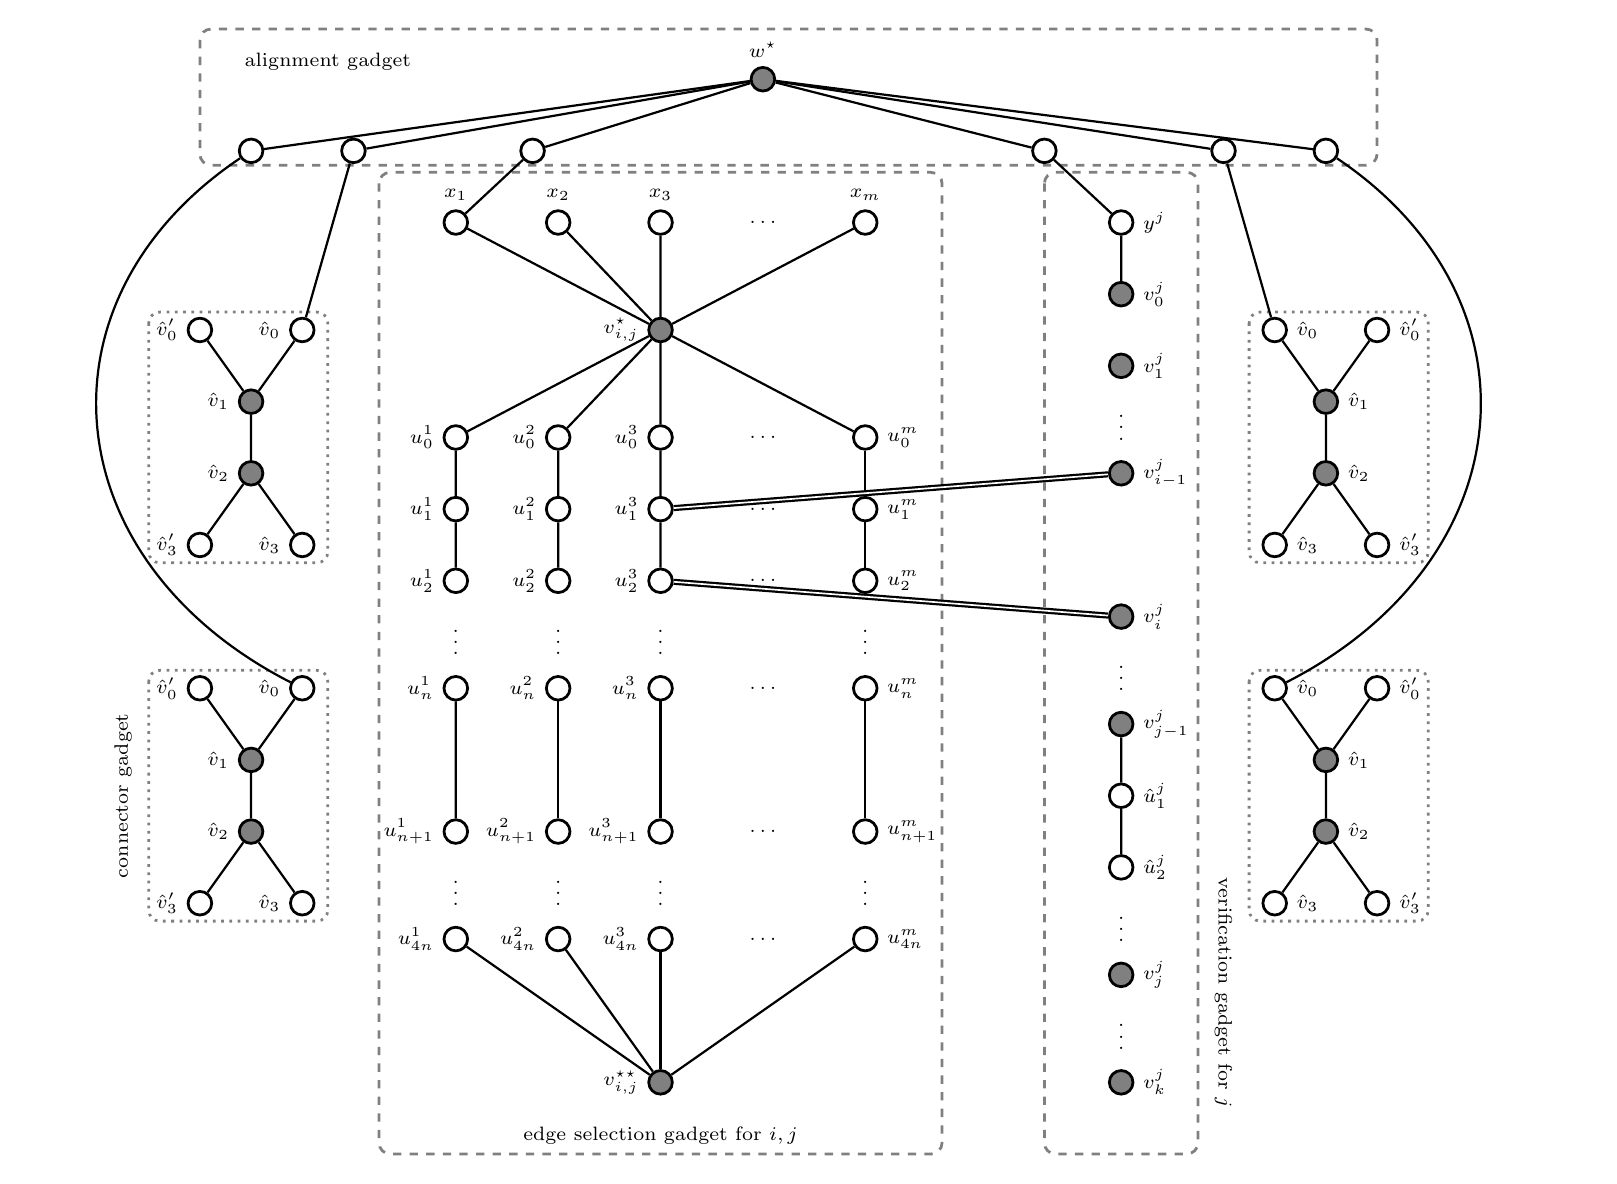
\begin{tikzpicture}[line width=1pt, scale=.65, yscale=.7]
\scriptsize
\node (A) at (14,0) {};

\draw[rounded corners, dashed, gray] (-13, 5.4) rectangle (10, 1.6) {};
\node (A) at (-10.5,4.5) {alignment gadget};

\draw[rounded corners, dotted, gray] (-14, -2.5) rectangle (-10.5, -9.5) {};
\draw[rounded corners, dotted, gray] (-14, -12.5) rectangle (-10.5, -19.5) {};
\draw[rounded corners, dotted, gray] (7.5, -2.5) rectangle (11, -9.5) {};
\draw[rounded corners, dotted, gray] (7.5, -12.5) rectangle (11, -19.5) {};
\node[rotate=90] (A) at (-14.5,-16) {connector gadget};

\draw[rounded corners, dashed, gray] (-9.5, 1.4) rectangle (1.5, -26) {};
\node (A) at (-4,-25.5) {edge selection gadget for $i,j$};

\draw[rounded corners, dashed, gray] (3.5, 1.4) rectangle (6.5, -26) {};
\node[rotate=-90] (A) at (7,-21.5) {verification gadget for $j$};

    \node[vert,label=above:$w^\star$, fill=gray] (W) at (-2,4) {};
    \node[vert] (W1) at (-6.5,2) {};
    \node[vert] (W2) at (-10,2) {};
    \node[vert] (W3) at (-12,2) {};
    \node[vert] (W4) at (7,2) {}; 
    \node[vert] (W5) at (3.5,2) {};
    \node[vert] (W6) at (9,2) {}; 


    \node[vert,label=left:$\hat{v}_0$] (VH11) at (-11,-3) {}; 
    \node[vert,label=left:$\hat{v}_0'$] (VH111) at (-13,-3) {}; 
    \node[vert,label=left:$\hat{v}_1$, fill=gray] (VH12) at (-12,-5) {}; 
    \node[vert,label=left:$\hat{v}_2$, fill=gray] (VH13) at (-12,-7) {}; 
    \node[vert,label=left:$\hat{v}_3$] (VH14) at (-11,-9) {};  
    \node[vert,label=left:$\hat{v}_3'$] (VH144) at (-13,-9) {}; 

    \node[vert,label=left:$\hat{v}_0$] (VH21) at (-11,-13) {};
    \node[vert,label=left:$\hat{v}_0'$] (VH211) at (-13,-13) {}; 
    \node[vert,label=left:$\hat{v}_1$, fill=gray] (VH22) at (-12,-15) {}; 
    \node[vert,label=left:$\hat{v}_2$, fill=gray] (VH23) at (-12,-17) {};
    \node[vert,label=left:$\hat{v}_3$] (VH24) at (-11,-19) {};
    \node[vert,label=left:$\hat{v}_3'$] (VH244) at (-13,-19) {}; 

    \node[vert,label=right:$\hat{v}_0$] (VH31) at (8,-3) {}; 
    \node[vert,label=right:$\hat{v}_0'$] (VH311) at (10,-3) {}; 
    \node[vert,label=right:$\hat{v}_1$, fill=gray] (VH32) at (9,-5) {}; 
    \node[vert,label=right:$\hat{v}_2$, fill=gray] (VH33) at (9,-7) {}; 
    \node[vert,label=right:$\hat{v}_3$] (VH34) at (8,-9) {};  
    \node[vert,label=right:$\hat{v}_3'$] (VH344) at (10,-9) {}; 

    \node[vert,label=right:$\hat{v}_0$] (VH41) at (8,-13) {}; 
    \node[vert,label=right:$\hat{v}_0'$] (VH411) at (10,-13) {}; 
    \node[vert,label=right:$\hat{v}_1$, fill=gray] (VH42) at (9,-15) {}; 
    \node[vert,label=right:$\hat{v}_2$, fill=gray] (VH43) at (9,-17) {}; 
    \node[vert,label=right:$\hat{v}_3$] (VH44) at (8,-19) {};  
    \node[vert,label=right:$\hat{v}_3'$] (VH444) at (10,-19) {}; 
    
    \node[vert,label=above:$x_1$] (X1) at (-8,0) {}; 
    \node[vert,label=above:$x_2$] (X2) at (-6,0) {}; 
    \node[vert,label=above:$x_3$] (X3) at (-4,0) {}; 
    \node (A) at (-2,0) {$\ldots$};
    \node[vert,label=above:$x_m$] (XM) at (0,0) {}; 
    
    \node[vert,label=left:$v_{i,j}^\star$, fill=gray] (VS) at (-4,-3) {}; 
    
    \node[vert,label=left:$u^1_0$] (Y1) at (-8,-6) {}; 
    \node[vert,label=left:$u^2_0$] (Y2) at (-6,-6) {}; 
    \node[vert,label=left:$u^3_0$] (Y3) at (-4,-6) {}; 
    \node (A) at (-2,-6) {$\ldots$};
    \node[vert,label=right:$u^m_0$] (YM) at (0,-6) {}; 

    \node[vert,label=left:$u^1_1$] (U11) at (-8,-8) {}; 
    \node[vert,label=left:$u^2_1$] (U12) at (-6,-8) {}; 
    \node[vert,label=left:$u^3_1$] (U13) at (-4,-8) {}; 
    \node (A) at (-2,-8) {$\ldots$};
    \node[vert,label=right:$u^m_1$] (U1M) at (0,-8) {};
    
    \node[vert,label=left:$u^1_2$] (U21) at (-8,-10) {}; 
    \node[vert,label=left:$u^2_2$] (U22) at (-6,-10) {}; 
    \node[vert,label=left:$u^3_2$] (U23) at (-4,-10) {}; 
    \node (A) at (-2,-10) {$\ldots$};
    \node[vert,label=right:$u^m_2$] (U2M) at (0,-10) {};
    
    \node (A) at (-8,-11.5) {$\vdots$}; 
    \node (A) at (-6,-11.5) {$\vdots$}; 
    \node (A) at (-4,-11.5) {$\vdots$}; 
    \node (A) at (0,-11.5) {$\vdots$};

    \node[vert,label=left:$u^1_n$] (UN1) at (-8,-13) {}; 
    \node[vert,label=left:$u^2_n$] (UN2) at (-6,-13) {}; 
    \node[vert,label=left:$u^3_n$] (UN3) at (-4,-13) {}; 
    \node (A) at (-2,-13) {$\ldots$};
    \node[vert,label=right:$u^m_n$] (UNM) at (0,-13) {};

    \node[vert,label=left:$u_{n+1}^1$] (UN11) at (-8,-17) {}; 
    \node[vert,label=left:$u_{n+1}^2$] (UN12) at (-6,-17) {}; 
    \node[vert,label=left:$u_{n+1}^3$] (UN13) at (-4,-17) {}; 
    \node (A) at (-2,-17) {$\ldots$};
    \node[vert,label=right:$u_{n+1}^m$] (UN1M) at (0,-17) {};
        
    \node (A) at (-8,-18.5) {$\vdots$}; 
    \node (A) at (-6,-18.5) {$\vdots$}; 
    \node (A) at (-4,-18.5) {$\vdots$}; 
    \node (A) at (0,-18.5) {$\vdots$};

    \node[vert,label=left:$u_{4n}^1$] (U2N1) at (-8,-20) {}; 
    \node[vert,label=left:$u_{4n}^2$] (U2N2) at (-6,-20) {}; 
    \node[vert,label=left:$u_{4n}^3$] (U2N3) at (-4,-20) {}; 
    \node (A) at (-2,-20) {$\ldots$};
    \node[vert,label=right:$u_{4n}^m$] (U2NM) at (0,-20) {};
    
    \node[vert,label=left:$v_{i,j}^{\star\star}$, fill=gray] (VSS) at (-4,-24) {};


    \node[vert,label=right:$y^j$] (YI) at (5,0) {};
    \node[vert,label=right:$v_0^j$, fill=gray] (VI0) at (5,-2) {};
    \node[vert,label=right:$v_1^j$, fill=gray] (VI1) at (5,-4) {};
    \node (A) at (5,-5.5) {$\vdots$};
    \node[vert,label=right:$v_{i-1}^j$, fill=gray] (VIJ1) at (5,-7) {};
    \node[vert,label=right:$v_{i}^j$, fill=gray] (VIJ) at (5,-11) {};
    \node (A) at (5,-12.5) {$\vdots$};
    \node[vert,label=right:$v_{j-1}^j$, fill=gray] (VII1) at (5,-14) {};
    \node[vert,label=right:$\hat{u}_{1}^j$] (UI1) at (5,-16) {};
    \node[vert,label=right:$\hat{u}_{2}^j$] (UI2) at (5,-18) {};
    \node (A) at (5,-19.5) {$\vdots$};
    \node[vert,label=right:$v_{j}^j$, fill=gray] (UIN3) at (5,-21) {};
    \node (A) at (5,-22.5) {$\vdots$};
    \node[vert,label=right:$v_{k}^j$, fill=gray] (VIK) at (5,-24) {};
    
	\draw[edge] (X1) --node[] {} (VS);
	\draw[edge] (X2) --node[] {} (VS);
	\draw[edge] (X3) --node[] {} (VS);
	\draw[edge] (XM) --node[] {} (VS);

    \draw[edge] (Y1) --node[] {} (VS);
	\draw[edge] (Y2) --node[] {} (VS);
	\draw[edge] (Y3) --node[] {} (VS);
	\draw[edge] (YM) --node[] {} (VS);

    \draw[edge] (Y1) --node[] {} (U11);
	\draw[edge] (Y2) --node[] {} (U12);
	\draw[edge] (Y3) --node[] {} (U13);
	\draw[edge] (YM) --node[] {} (U1M);
	
    \draw[edge] (U21) --node[] {} (U11);
	\draw[edge] (U22) --node[] {} (U12);
	\draw[edge] (U23) --node[] {} (U13);
	\draw[edge] (U2M) --node[] {} (U1M);

    \draw[edge] (UN1) --node[] {} (UN11);
	\draw[edge] (UN2) --node[] {} (UN12);
	\draw[edge] (UN3) --node[] {} (UN13);
	\draw[edge] (UNM) --node[] {} (UN1M);
 
    \draw[edge] (U2N1) --node[] {} (VSS);
	\draw[edge] (U2N2) --node[] {} (VSS);
	\draw[edge] (U2N3) --node[] {} (VSS);
	\draw[edge] (U2NM) --node[] {} (VSS);

    \draw[edge] (VH11) --node[] {} (VH12);
	\draw[edge] (VH12) --node[] {} (VH111);
	\draw[edge] (VH12) --node[] {} (VH13);
    \draw[edge] (VH13) --node[] {} (VH14);
	\draw[edge] (VH13) --node[] {} (VH144);
	
    \draw[edge] (VH21) --node[] {} (VH22);
	\draw[edge] (VH22) --node[] {} (VH211);
	\draw[edge] (VH22) --node[] {} (VH23);
    \draw[edge] (VH23) --node[] {} (VH24);
	\draw[edge] (VH23) --node[] {} (VH244);
 
    \draw[edge] (VH31) --node[] {} (VH32);
	\draw[edge] (VH32) --node[] {} (VH311);
	\draw[edge] (VH32) --node[] {} (VH33);
    \draw[edge] (VH33) --node[] {} (VH34);	
    \draw[edge] (VH33) --node[] {} (VH344);

    \draw[edge] (VH41) --node[] {} (VH42);
	\draw[edge] (VH42) --node[] {} (VH411);
	\draw[edge] (VH42) --node[] {} (VH43);
    \draw[edge] (VH43) --node[] {} (VH44);	
    \draw[edge] (VH43) --node[] {} (VH444);
 
	%\draw[edge] (VIJ1) --node[timelabel, near start] {$t_1+4$} (U13);
	%\draw[edge] (VIJ) --node[timelabel, near start] {$t_1+8$} (U23);

    \draw[edge,double] (VIJ1) --node {} (U13);
	\draw[edge,double] (VIJ) --node {} (U23);
 
 
	\draw[edge] (W) --node[] {} (W1);
	\draw[edge] (W) --node[] {} (W2);
	\draw[edge] (W) --node[] {} (W3);
	\draw[edge] (W) --node[] {} (W4);
	\draw[edge] (W) --node[] {} (W5);
	\draw[edge] (W) --node[] {} (W6);
 
	\draw[edge] (X1) --node[] {} (W1);
	\draw[edge] (VH11) --node[] {} (W2);
	\draw[edge] (VH21) edge[bend left=50] node[] {} (W3);
	\draw[edge] (VH31) --node[] {} (W4);
	\draw[edge] (YI) --node[] {} (W5);
	\draw[edge] (VH41) edge[bend right=50] node[] {} (W6);

	\draw[edge] (YI) --node[] {} (VI0);
 
	\draw[edge] (VII1) --node[] {} (UI1);
	\draw[edge] (UI1) --node[] {} (UI2);
\end{tikzpicture}
    %\end{center}
    }
    \caption{Illustration of part of the underlying graph $G$. Edges incident with vertices $\hat{v}_1,\hat{v}_2$ of connector gadgets are omitted. Gray vertices form a feedback vertex set.
    The double line connections, between a vertex $v_{i-1}^j$ in the verification gadget, and $u_1^3$ in the edge selection gadget, 
    and, between a vertex $u_2^3$ in the edge selection gadget, and $v_{i}^j$ in the verification gadget,
    consist of $5n$ vertices $a_1^{j,i,3},a_2^{j,i,3},\dots,a_{5n}^{j,i,3}$ 
    and $b_1^{j,i,3},b_2^{j,i,3},\dots,b_{5n}^{j,i,3}$, respectively.
    }\label{fig:hardness1}
\end{figure}


Furthermore, we use \emph{connector gadgets}, two for each edge selection gadget, and two for every verification gadget. They consist of six vertices $\hat{v}_0,\hat{v}_0',\hat{v}_1,\hat{v}_2,\hat{v}_3,\hat{v}_3'$ and, intuitively, are used to connect many vertex pairs by fast paths, which will make arguing about possible labelings in \textsc{Yes}-instances much easier. Finally, we have an \emph{alignment gadget}, which is a star with a center vertex $w^\star$ and a leaf for every other gadget. Intuitively, this gadget is used to relate labels of different gadgets to each other. A formal description of these two gadgets is given in the Appendix.

This finishes the description of the underlying graph $G$. For an illustration see \cref{fig:hardness1}. We can observe that the vertex set containing
%\begin{itemize}
 %   \item 
    vertices $v_{i,j}^\star$ and $v_{i,j}^{\star\star}$ of each edge selection gadget,
    %\item 
    vertices $v^i_\ell$ with $0\le \ell\le k$ of each verification gadget,
    %\item 
    vertices $\hat{v}_1$ and $\hat{v}_2$ of each connector gadget, and
    %\item 
    vertex $w^\star$ of the alignment gadget
%\end{itemize}
forms a feedback vertex set in $G$ with size $O(k^2)$.

As mentioned before, due to space constraints, we defer the description of the distance matrix $D$ and a formal correctness proof of the reduction to the Appendix.

\begin{comment}
\emph{Duration Matrix $D$.} We proceed with describing the matrix $D$ of durations of fastest paths. For a more convenient presentation, we use the notation $d(v,v'):= D_{v,v'}$. For all vertices $v,v'$ that are neighbors in $G$ we have that $d(v,v')=1$ and $d(v',v)=1$.

Next, consider a connector gadget consisting of vertices $\hat{v}_0,\hat{v}_0',\hat{v}_1,\hat{v}_2,\hat{v}_3,\hat{v}_3'$ and with sets $A$ and $B$. Informally, the connector gadget makes sure that all vertices in $A$ can reach all other vertices (of edge selection gadgets and validation gadgets) except the ones in $B$. We set the following durations. Recall that $V^\star$ denotes the set of all vertices from all edge selection gadgets and all validation gadgets.
\begin{itemize}
    \item We set $d(\hat{v}_0,\hat{v}_2)=d(\hat{v}_3,\hat{v}_1)=d(\hat{v}_2,\hat{v}_0')=d(\hat{v}_1,\hat{v}_3')=2$, and $d(\hat{v}_0,\hat{v}_0')=d(\hat{v}_3,\hat{v}_3')=d(\hat{v}_0,\hat{v}_3')=d(\hat{v}_3,\hat{v}_0')=3$.
    \item Let $v\in A$, then we set $d(v,\hat{v}_0')=3$ and $d(v,\hat{v}_3')=3$.
    \item Let $v\in V^\star\setminus B$, then we set $d(\hat{v}_0,v)=3$ and $d(\hat{v}_3,v)=3$.
    \item Let $v\in A$ and $v'\in V^\star\setminus B$ such that $v$ and $v'$ are not neighbors, then we set $d(v,v')=3$.
\end{itemize}
Now consider two connector gadgets, one with vertices $\hat{v}_0,\hat{v}_0',\hat{v}_1,\hat{v}_2,\hat{v}_3,\hat{v}_3'$ and with sets $A$ and $B$, and one with vertices $\hat{v}_0',\hat{v}_0'',\hat{v}_1',\hat{v}_2',\hat{v}_3',\hat{v}_3''$ and with sets $A'$ and $B'$.
\begin{itemize}
    \item If there is a vertex $v\in A$ with $v\notin A'$, then we set $d(\hat{v}_1,\hat{v}_1')=3$.
    \item If there is a vertex $v\in A$ with $v\in A'\setminus B'$, then we set $d(\hat{v}_1,\hat{v}_2')=3$.
    \item If there is a vertex $v\in V^\star\setminus (A\setminus B)$ with $v\notin A'$, then we set $d(\hat{v}_2,\hat{v}_1')=3$.    
    \item If there is a vertex $v\in V^\star\setminus (A\setminus B)$ with $v\in A'\setminus B'$, then we set $d(\hat{v}_2,\hat{v}_2')=3$.
\end{itemize}

Next, consider the edge selection gadget for color combination $i,j$ with $i<j$.
\begin{itemize}
    \item Let $1\le \ell<\ell'\le m$. We set $d(x_\ell,x_{\ell'})=2n\cdot (i+j)\cdot((\ell')^2-\ell^2)+1$.
    \item For all $\ell\in[m]$ we set $d(x_\ell,v_{i,j}^{\star\star})=8n+5$.
\end{itemize}

Next, consider the validation gadget for color $i$. 
%Let $1\le j<i$, let $e_\ell\in F_{j,i}$, and let $w^i_{\ell'}\in W_i$ be incident with $e_\ell$. We set the following.
%\begin{itemize}
    %\item We set $d(v^i_{j-1},w^i_{\ell'+1})=3$.
    %\item We set $d(w^i_{\ell'},v^i_{j})=3$.
%\end{itemize}
%
For all $0\le j<j'<i$ and all $i\le j<j'\le k$ we set the following.
\begin{itemize}
    \item We set $d(v^i_j,v^i_{j'})=(20n+6)(j'-j)-1$.
\end{itemize}
%The next cases are only relevant if $1\neq i \neq k$. 
%For all $0\le j<i$ %and $\ell\in[n+3]$ we set the following.
%\begin{itemize}
%    \item We set $d(v^i_j,\hat{u}^i_{n+3})=(20n+6)(i-j-1)+2n+5$.
%\end{itemize}
%For all $\ell,\ell'\in[n+3]$ with $\ell<\ell'$ we set the following.
%\begin{itemize}
%    \item We set $d(\hat{u}^i_{\ell},\hat{u}^i_{\ell'})=2(\ell'-\ell)-1$.
%\end{itemize}
For all $0\le j<i$ and all $i\le j'\le k$ we set the following.
\begin{itemize}
    \item We set $d(v^i_j,v^i_{j'})=(20n+6)(j'-j)+6n-1$.
\end{itemize}
%For all 
%$\ell\in[n+3]$ and 
%$i<j\le k$ we set the following.
%\begin{itemize}
%    \item We set $d(\hat{u}^i_{n+3},v^i_j)=(20n+6)(j-i)-1$.
%\end{itemize}

Finally, we consider the alignment gadget. Let $x_1$ belong to the edge selection gadget of color combination $i,j$ and let $w\in \hat{W}$ denote the neighbor of $x_1$ in the alignment gadget. Let $\hat{v}_1$ and $\hat{v}_2$ belong to the first connector gadget of the edge selection gadget for color combination $i,j$. Let $\hat{V}$ contain all vertices $\hat{v}_1$ and $\hat{v}_2$ belonging to the other connector gadgets (different from the first one of the edge selection gadget for color combination $i,j$). 
\begin{itemize}
    \item We set $d(w^\star,x_1)=(20n+6)(i+j)$.
    \item We set $d(w^\star,\hat{v}_1)=n^9$, $d(w,\hat{v}_2)=n^9$, $d(w,\hat{v}_1)=n^9-(20n+6)(i+j)+1$, and $d(w,\hat{v}_2)=n^9-(20n+6)(i+j)+1$.
    \item For each vertex $v\in (V^\star\cup \hat{V})\setminus (X_{i,j}\cup \{v_{i,j}^{\star\star}\})$ we set $d(w^\star,v)=n^9+2$ and $d(w,v)=n^9-(20n+6)(i+j)+3$.
\end{itemize}

Let $y^i$ belong to the verification gadget of color $i$ and let $w'\in \hat{W}$ denote the neighbor of $y^i$ in the alignment gadget. Let $\hat{v}_1$ and $\hat{v}_2$ belong to the connector gadget of the verification gadget for color $i$. Let $\hat{V}$ contain all vertices $\hat{v}_1$ and $\hat{v}_2$ belonging to the other connector gadgets (different from the one of the verification gadget for color $i$). Let $V_i$ denote the set of all vertices of the verification gadget of color $i$.
\begin{itemize}
    \item We set $d(w^\star,y^i)=n^8-1$, $d(w',v^i_0)=2$, and $d(w^\star,v^i_0)=n^8$.
    \item We set $d(w^\star,\hat{v}_1)=n^9$, $d(w^\star,\hat{v}_2)=n^9$, $d(w',\hat{v}_1)=n^9-n^8$, and $d(w',\hat{v}_2)=n^9-n^8$.
    \item For each vertex $v\in (V^\star\cup \hat{V})\setminus V_i$ we set $d(w^\star,v)=n^9+1$, $d(w,v)=n^9-n^8+2$, and $d(y^i,v)=n^9-n^8+2$.
\end{itemize}
Let $\hat{v}_1$ belong to some connector gadget. Then we set $d(w^\star,\hat{v}_1)=n^9$.

All fastest path durations between non-adjacent vertex pairs that are not specified above are set to infinity.

\end{comment}

%This finishes the construction of \deltaExactLong\ instance $D$, which can clearly be computed in polynomial time. For an illustration see \cref{fig:hardness1}. As discussed earlier, we have that the vertex cover number of the underlying graph of the instance is in $O(k^2)$.


%
%\begin{comment}
\emph{Infinity gadget.} Finally, we show how to get rid of the infinity entries in $D$ and how to allow a finite $\Delta$. To this end, we introduce the \emph{infinity gadget}. We add four vertices $z_1, z_2, z_3, z_4$ to the graph and we set $\Delta=n^{11}$. Let $V$ denote the set of all remaining vertices. We set the following durations.
\begin{itemize}
    \item For all $v\in V$ we set $d(z_1,v)=2$, $d(z_2,v)=d(v,z_2)=1$, $d(z_3,v)=d(v,z_3)=1$, and $d(z_4,v)=2$.
    Furthermore, we set $d(v,z_1)=n^{11}$ and $d(v,z_4)=n^{10}-1$.
    \item We set $d(z_1,z_2)=d(z_2,z_1)=1$, $d(z_2,z_3)=d(z_3,z_2)=1$, and $d(z_3,z_4)=d(z_4,z_3)=1$.
    \item We set $d(z_1,z_3)=3$, $d(z_3,z_1)=n^{11}-1$, $d(z_2,z_4)=n^{10}-2$, and $d(z_4,z_2)=n^{11}-n^{10}+4$.
    \item We set $d(z_1,z_4)=n^{10}$ and $d(z_4,z_1)=2n^{11}-n^{10}+2$.
    \item For every pair of vertices $v,v'\in V$ where previously the duration of a fastest path from $v$ to $v'$ was specified to be infinite, we set $d(v,v')=n^{10}$.
\end{itemize}
Now we analyse which implications we get for the labels on the newly introduced edges.
Assume $\lambda(\{z_1,z_2\})=t$, then we get the following.
%\begin{itemize}
    %\item 
    For all $v\in V$ we have that $d(z_1,v)=2$ and hence we get that $\lambda(\{z_2,v\})=t+1$. 
    %\item 
    Since $d(z_1,z_4)=n^{10}$, we have that $\lambda(z_3,z_4)=t+n^{10}-1$.
    From this follows that for all $v\in V$, since $d(z_4,v)=2$, that $\lambda(\{z_3,v\})=t+n^{10}$.
    Finally, since $d(z_1,z_3)=3$, we have that $\lambda(\{z_2,z_3\})=t+2$.
%\end{itemize}
For an illustration see \cref{fig:hardness2}. It is easy to check that all duration requirements between vertex pairs in $\{z_1,z_2,z_3,z_4\}$ are met and that all duration requirements between each vertex $v\in V$ and each vertex in  $\{z_1,z_2,z_3,z_4\}$ are met. Furthermore, it is easy to check that the gadget increases the feedback vertex set by two ($z_2$ and $z_3$ need to be added).

\begin{figure}[t]
%\noindent\makebox[\textwidth]{
\centering
%\begin{center}
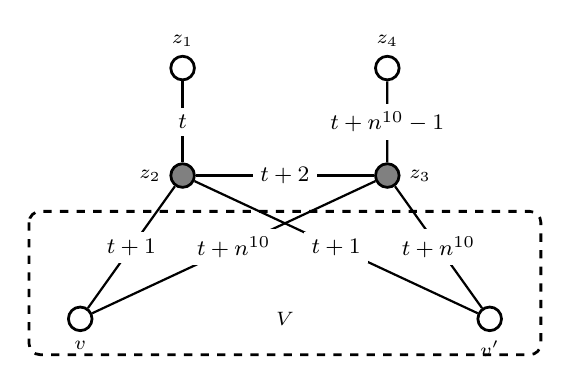
\begin{tikzpicture}[line width=1pt, scale=.65,yscale=.7]
\scriptsize


\draw[rounded corners, dashed] (-3, -4) rectangle (7, -8) {};
\node (A) at (2,-7) {$V$};

    \node[vert,label=above:$z_1$] (Z1) at (0,0) {};
    \node[vert,label=left:$z_2$, fill=gray] (Z2) at (0,-3) {};
    \node[vert,label=right:$z_3$, fill=gray] (Z3) at (4,-3) {};
    \node[vert,label=above:$z_4$] (Z4) at (4,0) {};
    
    \node[vert,label=below:$v$] (V) at (-2,-7) {};
    \node[vert,label=below:$v'$] (VV) at (6,-7) {};

    \draw[edge] (Z1) --node[timelabel] {$t$} (Z2);
    \draw[edge] (Z2) --node[timelabel] {$t+2$} (Z3);
    \draw[edge] (Z3) --node[timelabel] {$t+n^{10}-1$} (Z4);

    \draw[edge] (Z2) --node[timelabel] {$t+1$} (V);
    \draw[edge] (Z3) --node[timelabel] {$t+n^{10}$} (V);
    \draw[edge] (Z2) --node[timelabel] {$t+1$} (VV);
    \draw[edge] (Z3) --node[timelabel] {$t+n^{10}$} (VV);
\end{tikzpicture}
    %\end{center}
%    }
    \caption{Illustration of the infinity gadget. Gray vertices are added to the feedback vertex set.}\label{fig:hardness2}
\end{figure}

Lastly, consider two vertices $v,v'\in V$. Note that before the addition of the infinity gadget, by construction of $G$ we have that $d(v,v')\le n^9+2$ or $d(v,v')=\infty$. Furthermore, if $D$ is a \textsc{Yes}-instance, we have shown in the correctness proof of the reduction that the difference between the smallest label and the largest label is at most $n^9+1$. This implies that for a vertex pair $v,v'\in V$ with $d(v,v')=\infty$ we have in the periodic case with $\Delta=n^{11}$, that $d(v,v')\ge n^{11}-n^9>n^{10}$. Which means, after adding the vertices and edges of the infinity gadget, we indeed have that $d(v,v')=n^{10}$. For all vertex pairs $v,v'$ where in the original construction we have $d(v,v')\neq\infty$, we can also see that adding the infinity gadget and setting $\Delta=n^{11}$ does not change the duration of a fastest path from $v$ to $v'$, since all newly added temporal paths have duration at least $n^{10}$. We can conclude that the originally constructed instance $D$ is a \textsc{Yes}-instance if and only if it remains a \textsc{Yes}-instance after adding the infinity gadget and setting $\Delta=n^{11}$.
%\end{comment}
\end{proof}


%\pagebreak

\section{Algorithms for \deltaExact}
\begin{comment}
In this section we provide several algorithms for \deltaExact. By \cref{thm:NPhardness} we have that \deltaExact\ is NP-hard in general, hence we start by identifying restricted cases where we can solve the problem in polynomial time.
%
The first case, when the underlying graph $G$ of an instance $(D, \Delta)$ of \deltaExact\ is a tree, we get the following result. 

\begin{theorem}[$\star$]\label{thm:deltaExact-PolyTimeTrees}
    \deltaExact\ can be solved in polynomial-time on trees.
\end{theorem}

In the case when the underlying graph is unrestricted, we show that \deltaExact\ is fixed-parameter tractable when parameterized by the feedback edge number of the underlying graph. Note that our parameterized hardness result (\cref{thm:W1wrtFVS}) implies that we presumably cannot replace the feedback edge number with the smaller parameter feedback vertex number, or any other parameter that is smaller than the feedback vertex number, such as e.g.\ the treewidth.
In the Appendix we give also a dedicated algorithm to solve \deltaExact\ in polynomial time if the underlying graph is a cycle. Note that this is already implied by our FPT result, however the direct algorithm we provide is much simpler for this case.
\end{comment}

In this section we provide several algorithms for \deltaExact. By \cref{thm:NPhardness} we have that \deltaExact\ is NP-hard in general, hence we start by identifying restricted cases where we can solve the problem in polynomial time.
We first show in \cref{sec:treealgo} that if the underlying graph $G$ of an instance $(D, \Delta)$ of \deltaExact\ is a tree, then we can determine desired $\Delta$-periodic labeling $\lambda$ of $G$ in polynomial time. In \cref{sec:FPT} we generalize this result. We show that \deltaExact\ is fixed-parameter tractable when parameterized by the feedback edge number of the underlying graph. Note that our parameterized hardness result (\cref{thm:W1wrtFVS}) implies that we presumably cannot replace the feedback edge number with the smaller parameter feedback vertex number, or any other parameter that is smaller than the feedback vertex number, such as e.g.\ the treewidth.
%In the appendix we give a dedicated algorithm to solve \deltaExact\ in polynomial time if the underlying graph is a cycle. Note that this is already implied by our FPT result, however the direct algorithm we provide is much simpler for this case.



%We first start with defining certain notions, that will be of use when solving the problem.

%    \begin{definition}[Travel delays]
%    Let $(G, \lambda)$ be a temporal graph satisfying conditions of \deltaExact.
%    Let $e_1=uv$ and $e_2=vz$ be two incident edges in $G$ with $e_1 \cap e_2 = v$.
%    We define the \emph{travel delay} from $u$ to $z$ at vertex $v$, denoted with $\tau_v^{uz}$,
%    as the difference of the labels of $e_2$ and $e_1$, where we subtract the value of the label of $e_1$ from the label of $e_2$,  modulo~$\Delta$.
%    More specifically:
%    \begin{equation}\label{eq:def-VertexWaitingTime}
%       \tau_v^{uz} \equiv \lambda (e_2) - \lambda(e_1) \pmod \Delta.
%    \end{equation}
%    Similarly, $\tau_v^{zu} \equiv \lambda (e_1) - \lambda(e_2) \pmod \Delta$.
%    \end{definition}
%    Intuitively, the value of $\tau_v^{uz}$ represents how long a temporal path waits at vertex $v$ when first taking edge $e_1=uv$ and then edge $e_2 = vz$.

%    We can make the following observation concerning subpaths of a fastest temporal path.

%\begin{lemma}[$\star$]\label{lemma:unique-fastest-path-allDelays}
%    Let $(G, \lambda)$ be a temporal graph satisfying conditions of the \deltaExact\ problem,
%    and let $(P_{1,k},\lambda)$ be a fastest temporal path from $u=v_1$ to $v=v_k$ on $k$ vertices $v_1,v_2,\dots,v_k$.
%    Let us denote with $(P_{1,i}, \lambda)$ the sub-path of temporal path $(P_{1,k},\lambda)$, that starts at $v_1$ and finishes at $v_i$.
%    Suppose that, for any $v_i$ in $P$, we have that $(P_{1,i}, \lambda)$ is also the fastest temporal path from $u=v_1$ to $v_i$.
%    Then we can determine travel delays on vertices of $P$ using the following equation
%    \begin{equation}\label{eq:trav-delays-paths}
%        \tau_{v_i}^{v_{i-1},v_{i+1}} = D_{1,i+1} - D_{1,i},
%    \end{equation}
%    for all $i \in \{2,3, \dots, k-1\}$.
%\end{lemma}




\subsection{Polynomial-time algorithm for trees}\label{sec:treealgo}
%All of the above is used in the design of the following polynomial-time algorithms.
We now provide a polynomial-time algorithm for \deltaExact\ when the underlying graph is a tree.
Let $D$ be the input matrix and let the underlying graph $G$ of $D$ be a tree on $n$ vertices $\{v_1, v_2, \dots, v_n\}$.
Let $v_i,v_j$ be two arbitrary vertices in $G$, then we know that there exists a unique (static) path $P_{i,j}$ from $v_i$ to $v_j$. We will heavily exploit this in our algorithm.
%Consequently, the temporal path $(P_{i,j},\lambda)$ from $v_i$ to $v_j$ is also unique, up to modulo of the period $\Delta$ of the labeling $\lambda$,
%and therefore are the fastest.
%Then $D$ is of the following form:
%\begin{equation*}
%    D_{i,j} =
%    \begin{cases}
%    0 & \text{if $i = j$}, \\
%    1 & \text{if $v_i$ and $v_j$ are neighbours in G}\\
%    d(P_{i,j},\lambda) & \text{else}
%    \end{cases},
%\end{equation*}
%where $d(P_{i,j},\lambda)$ is the duration of the (unique) temporal path $(P_{i,j},\lambda)$ from $v_i$ to $v_j$.

%\begin{observation}\label{obs:travel-delays-in-trees}
%    Let $v_i,v_j$  be arbitrary two vertices in a tree $G$. 
%    Since there is a unique temporal path $(P_{i,j},\lambda)$ from $v_i$ to $v_j$, it is also the fastest one, therefore $d(P_{i,j},\lambda) = D_{i,j}$. 
%    Note, all other vertices $v' \in P_{i,j} \setminus \{v_i,v_j\}$ are reached form $v_i$ using a part of the path $(P_{i,j},\lambda)$.
%    \end{observation}
%    Now using \cref{lemma:unique-fastest-path-allDelays}, we can determine the waiting times for all \emph{inner} vertices of $P_{i,j}$.


\begin{theorem} \label{thm:deltaExact-PolyTimeTrees}
    \deltaExact\ can be solved in polynomial time on trees.
\end{theorem}

\begin{proof}
    Let $D$ be an input matrix for problem \deltaExact\ of dimension $n \times n$.
    Let us fix the vertices of the corresponding graph $G$ of $D$ as $v_1, v_2, \dots, v_n$, where vertex $v_i$ corresponds to the row and column $i$ of matrix $D$.
    This can be done in polynomial time as we need to loop through the matrix $D$ once and connect vertices $v_i, v_j$ for which $D_{i,j} = 1$. At the same time we also check if $D_{i,i} = 0$, for all $i \in [n]$.
    When $G$ is constructed we run DFS algorithm on it and check that it has no cycles.
    If at any step we encounter a problem, our algorithm stops and returns a negative answer.

    Having computed $G$, our algorithm proceeds as follows. We pick an arbitrary edge $f$ and give it label one, that is, $\lambda(f)=1$. Now we push all edges incident with $f$ into a (initially empty) queue. Now we repeat the following as long as the queue is not empty:
\begin{itemize}
    \item Pop edge $e=\{u,v\}$ from the queue. Since $e$ was pushed into the queue, there is an edge $e'$ incident with $e$ that already obtained a label. Let w.l.o.g.\ $e'=\{v,w\}$. Then we set $\lambda(e)=(\lambda(e')-D_{u,w}+1)\bmod \Delta$.
    \item Push all edges incident with $e$ that have not received a label yet into the queue.
\end{itemize}
When the queue is empty, all edges have received a label. Iterate over all vertex pairs $u,v$ and check whether the fastest path from $u$ to $v$ in $(G,\lambda)$ has duration $D_{u,v}$. If this check succeeds for all vertex pairs, output the labelling $\lambda$, otherwise abort.

It is easy to see that the described algorithm runs in polynomial time. In the remainder, we proof that it is correct.

$(\Rightarrow)$: Since the algorithm checks at the end whether all durations specified in $D$ are realized by the corresponding fastest paths, we clearly face a yes-instance whenever the algorithm outputs a labeling.

$(\Leftarrow)$: Assume we face a yes-instance, then there exists a labeling $\lambda^\star$ that realizes all durations specified in $D$. Let $e^\star$ denote the edge initially picked by the algorithm. For all edges $e$ let $\lambda(e)=(\lambda^\star(e)-\lambda^\star(e^\star)+1)\bmod \Delta$. Clearly, the labeling $\lambda$ also realizes all durations specified in $D$ since $\lambda$ is obtained by adding the constant $(1-\lambda^\star(e^\star))$ modulo $\Delta$ to all labels of $\lambda^\star$ which does not change the duration of any temporal path, that is all durations in $(G,\lambda^\star)$ are the same as their counterparts in $(G,\lambda)$. We claim that our algorithm computes and outputs $\lambda$.

We prove that our algorithm computes $\lambda$ by induction on the distance of the labeled edges to $e^\star$, where the distance of two edges $e,e'$ is defined as the length of a shortest path that uses $e$ as its first edge and $e'$ as its last edge.

Initially, our algorithm labels $e^\star$ with one, which equals $\lambda(e^\star)$. Now let $e$ be an edge popped off the queue by the algorithm in some iteration. Let $e'$ be the edge incident with $e$ that already obtained a label and is considered by the algorithm. Since $G$ is a tree, we have that $e'$ is closer to $e^\star$ than $e$. By induction we have that the algorithm labeled $e'$ with $\lambda(e')$. 
Assume that $e=\{u,v\}$ and $e'=\{v,w\}$. Since $G$ is a tree there is only one path from $u$ to $w$ in $G$ and it uses edges $e$ and $e'$. It follows that $\lambda(e')-\lambda(e)+1=D_{u,w}$ if $\lambda(e')>\lambda(e)$, and $\lambda(e')-\lambda(e)+\Delta+1=D_{u,w}$ otherwise. Our algorithm labels $e$ with $(\lambda(e')-D_{u,w}+1)\bmod \Delta$. It is straightforward to verify that the label of $e$ computed by the algorithm equals $\lambda(e)$. It follows that the algorithm computes $\lambda$.
%    From now on we can assume that we know that the underlying graph $G$ of $D$ is a tree and we know its structure.
%    For the next part of the algorithm we use \cref{obs:travel-delays-in-trees}.
%    
%    We pick an arbitrary vertex $v_i \in V(G)$ and check which vertex $v_j \in V(G)$ is furthest away from it, \ie we find a maximum element in the $i$-th row of the matrix $D$.
%    We now take the unique path $P_{i,j}$ in $G$, 
%    which has to also be the underlying path of the fastest temporal path from $v_i$ to $v_j$, and using \cref{obs:travel-delays-in-trees} calculate waiting times at all inner vertices.
%    We save those values in a matrix $T$, of size $n \times n \times n$, and mark vertices of the path  $P_{i,j}$ as visited.
%    Matrix $T$ stores at the position $(k,j,\ell)$ the value corresponding to the travel delay at vertex $v_k$ when traveling from $v_{j}$ to $v_{\ell}$, 
%    \ie it stores the value $\tau_{v_k}^{v_{j}, v_\ell}$, where $v_j,v_\ell \in N(v_k)$. All other values of $T$ are set to \textsc{Null}.
%    Now we repeat procedure, from vertex $v_i$, for vertices that are not marked as visited yet, \ie vertices in $V \setminus P_{i,j}$.
%    We find a vertex in $V \setminus P_{i,j}$ that is furthest away from $v_i$ and repeat the procedure.
%    When we have exhausted the $i$-th row of $D$,
%    \ie vertex $v_i$ now reaches every vertex of $G$,
%    we continue and repeat the procedure for all other vertices.
%    If at any point we get two different values for the same travel delay at a specific vertex, then we stop with the algorithm and return the negative answer.
%    If the above procedure finishes successfully we get the matrix $T$ with travel delays for all vertices in $G$, of degree at least $2$.
%    The above calculation is performed in polynomial time, as for every vertex $v_i$ we inspect the whole graph once.
%    \begin{claim}[$\star$]\label{lemma:matrixT-travelDelays-tree}
%        Matrix $T$ consists of travel delays for all vertices of degree at least $2$ in $G$.
%    \end{claim}
%
%
%    Now, given the matrix of travel delays $T$, we can find a labeling $\lambda$ that satisfies $D$.
%    We start by fixing the label of an arbitrary edge as $a$, where $a \in [\Delta]$.
%    Knowing the label of one edge, and all waiting times in $T$, we can uniquely determine the labels of all other edges.
%    More specifically, if we know that $\lambda(v_i v_j) = a$, then for all $v_k \in N(v_i)$ (resp.~$v_{k'} \in N(v_j)$)
%    the value $\lambda(v_iv_k) \equiv a + \tau_{v_i}^{v_j,v_k} \pmod \Delta $ (resp.~$\lambda(v_j v_{k'}) \equiv a + \tau_{v_j}^{v_i,v_{k'}} \pmod \Delta $).
%    Since there are $\Delta$ options to fix the first label, we can find $\Delta$ different labelings satisfying $D$.
%    Note, w.l.o.g. we can start determining the labeling $\lambda$ by setting $\lambda(v_1v_2) = 1$.
%    It is not hard to see, that also the calculation of the labeling $\lambda$ takes polynomial time, as we have to traverse the graph exactly once, to successfully fix the labeling. Therefore, all together the whole algorithm is performed in polynomial time.
\end{proof}







\subsection{FPT-algorithm for feedback edge number}\label{sec:FPT}

Recall from \cref{sec:treealgo} that the main reason, for which \deltaExact\ is straightforward to solve on trees, is twofold: 
\begin{itemize}
    \item between any pair of vertices $v_i$ and $v_j$ in the tree $T$, there is a \emph{unique} path $P$ in $T$ from $v_i$ to $v_j$, and 
    \item in any periodic temporal graph $(T,\lambda,\Delta)$ and any fastest temporal path $P=((e_1,t_1),\ldots,(e_i,t_i),\ldots,(e_j,t_j),\ldots,(e_\ell,t_\ell))$ from $v_1$ to $v_{\ell}$ we have that the sub-path $P'=((e_i,t_i),\ldots,(e_j,t_j))$ is also a fastest temporal path from $v_i$ to $v_j$.
\end{itemize}
However, these two nice properties do not hold when the underlying graph is not a tree. For example, in~\cref{fig:ftpExample}, the fastest temporal path from $u$ to $v$ is $P_{u,v}$ (depicted in blue) goes through~$w$, however the sub-path of $P_{u,v}$ that stops at $w$ is not the fastest temporal path from $u$ to $w$. The fastest temporal path from $u$ to $w$ consists only of the single edge $uw$ (with label $9$ and duration $1$, depicted in red).
%, while the fastest temporal path from $u$ to $v$ contains the four other edges (with labels 1, 3, 5, 7 and duration 7). 

Nevertheless, we prove in this section that we can still solve \deltaExact\ efficiently if the underlying graph is similar to a tree; more specifically we show the following result, which turns out to be non-trivial.

% In this section we show how to generalize the polynomial-time algorithm for trees. Following the \emph{distance-from-triviality} parameterization paradigm~\cite{FJR13,GHN04}, we aim to obtain fixed-parameter tractability using a parameter that measures the distance from the underlying graph to a tree. \cref{thm:W1wrtFVS} tells us that we presumably cannot use the feedback vertex number (or any smaller measure such as the treewidth) as a parameter to obtain tractability. Hence, we choose the feedback edge number as a parameter and we present an FPT algorithm for \deltaExact\ parameterized by the feedback edge number of the underlying graph.

% In a graph $G=(V,E)$, a \emph{feedback edge set} $F \subseteq E(G)$ is a subset of edges, such that each cycle in $G$ has at least one edge in $F$. The minimum such set $F$ is called a  \emph{minimum feedback edge set} and its size, $k = |F|$, is called the \emph{feedback edge number} of graph $G$. Determining $F$ can be done in linear time, by simply removing edges of a spanning tree (forest) from the given graph.
%one can find a minimum feedback edge set in linear time, by calculating a spanning tree (or forest) $T$ of the given graph $G$ and then removing all of the edges $T$ from $G$.%, \ie $F = E(G) \setminus E(T)$.

	\begin{figure}[t]
    \centering
	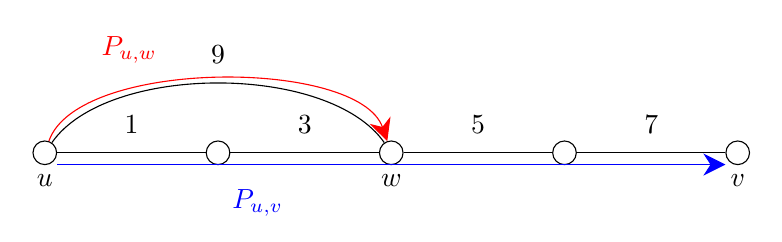
\begin{tikzpicture}[xscale=2.2,yscale=0.5]
	%%%S_uv
	\node[vert,label=below:$u$] (v1) at (1,0) {};
	\node[vert] (v2) at (2,0) {};
	\node[vert,label=below:$w$] (v3) at (3,0) {};
	\node[vert] (v4) at (4,0) {};
	\node[vert,label=below:$v$] (v5) at (5,0) {};

	\draw[transform canvas={yshift=-1.5mm}, blue]
	(v1) edge[diredge2]  node[pos=0.3,yshift=-2,label=below:$P_{u,v}$] {} (v5) ;
	
	\draw[red]
	(v1) edge[diredge2] [out=85,in=95,distance=2.1cm] node[pos=0.3,yshift=2,label=above:$P_{u,w}$] {} (v3) ;
 
	\draw (v1) -- node[label=above:$1$] {} (v2) -- node[label=above:$3$] {}  (v3) -- node[label=above:$5$] {} (v4) -- node[label=above:$7$] {} (v5);
	\draw (v1) to [out=80,in=100,distance=2cm] node[label=above:$9$] {} (v3);
	

\end{tikzpicture}
	\caption{An example of a temporal graph (with $\Delta \geq 9$), where the fastest temporal path $P_{u,v}$ (in blue) from $u$ to $v$ is of duration $7$,
		while the fastest temporal path $P_{u,w}$ (in red) from $u$ to a vertex $w$, that is on a path $P_{u,v}$, is of duration $1$ and is not a subpath of $P_{u,v}$.		
		\label{fig:ftpExample}}
	\end{figure}

\begin{theorem}[$\star$]\label{thm:FPTwrtFES}
    \deltaExact\ is in FPT when parameterized by the feedback edge number of the underlying graph.
\end{theorem}

From \cref{thm:W1wrtFVS} and \cref{thm:FPTwrtFES} we immediately get the following, which is the main result of the paper.

\begin{corollary}
\deltaExact\ is:
\begin{itemize}
    \item in FPT when parameterized by the \emph{feedback edge number} or any larger parameter, such as the \emph{maximum leaf number}.
    \item W[1]-hard when parameterized by the \emph{feedback vertex number} or any smaller parameter, such as: 
    \emph{treewidth}, 
    \emph{degeneracy}, 
    \emph{cliquewidth}, 
    \emph{distance to chordal graphs}, and 
    \emph{distance to outerplanar graphs}.
\end{itemize}
\end{corollary}

Before presenting the structure of our algorithm for \cref{thm:FPTwrtFES}, observe that, in a static graph, the number of paths between two vertices can be upper-bounded by a function $f(k)$ of the feedback edge number $k$ of the graph. 
Therefore, for any fixed pair of vertices $u$ and $v$, we can ``guess'' the edges of the fastest temporal path from $u$ to $v$. 
However, 
% due to the difficulties illustrated in~\cref{fig:ftpExample}, 
for an FPT algorithm with respect to $k$, we cannot afford to guess the edges of the fastest temporal path for each of the $O(n^2)$ pairs of vertices. 
To overcome this difficulty, our algorithm follows this high-level strategy:
\begin{itemize}
    %%%\item We perform a preprocessing step by iteratively removing all vertices of degree one.
    \item We identify a small number $f(k)$ of ``important vertices''; these consist of the sets that we call $U, U^{\ast}, Z^{\ast}$.
    \item For each pair $u,v$ of important vertices, we guess the edges of the fastest temporal path from $u$ to $v$ (and from $v$ to $u$).
    \item From these guesses we can still not deduce the edges of the fastest temporal paths between many pairs of non-important vertices. However, as we prove, it suffices to guess only a small number of specific auxiliary structures (to be defined later).
    \item From these guesses we deduce fixed relationships between the labels of most of the edges of the graph. 
    \item For all the edges, for which we do not have deduced a label yet, we introduce a \emph{variable}. Using all these variables, we build an Integer Linear Program (ILP). 
    Among the constraints in this ILP we have that, for each of the $O(n^2)$ pairs of vertices $u,v$ in the graph, the duration of one specific temporal path from $u$ to $v$ (according to our guesses) is \emph{equal} to the desired duration $D_{u,v}$, while the duration of each of the other temporal paths from $u$ to $v$ is \emph{at least} $D_{u,v}$.
    \item By making any of the above guesses, we restrict the solution space for the problem \deltaExact. This restricted solution space coincides with the set of feasible solutions to the resulting ILP. Furthermore, the set of feasible solutions for all constructed ILPs coincide with the set of all solutions to \deltaExact\ (\ie regardless of our guesses). As each ILP can be solved in FPT time with respect to $k$ by Lenstra's Theorem~\cite{Lenstra1983Integer} (the number of variables is upper bounded by a function of $k$), we obtain our FPT algorithm for \deltaExact\ with respect to $k$.
\end{itemize}


We now present the first part of our FPT algorithm, that is, identifying important vertices and guessing information about the fastest temporal paths. A full description of the algorithm is deferred to the Appendix.

\subparagraph{Important vertices.}
Let $D$ be the input matrix of \deltaExact\, and let $G$ be its underlying graph, on $n$ vertices and $m$ edges.
%\subsubsection*{Preprocessing of the input}
From the underlying graph $G$ of $D$ we first create a graph $G'$ by
iteratively removing vertices of degree one from $G$,
and denote with 
$
Z = V(G) \setminus V(G')
$, the set of removed vertices.
%Then we determine a minimum feedback edge set $F$ of $G'$.
%by finding a spanning tree $T$ of $G'$ and set $F = E(G) \setminus E(T)$. 
%Note that $F$ is also a minimum feedback edge set of $G$.
Then we determine the set $U$ (the \emph{``vertices of interest''}), and the set $U^*$ (the neighbors of the vertices of interest), as follows.
Let $T$ be a spanning tree of $G'$, with $F$ being the corresponding feedback edge set of $G'$.
Let $V_1 \subseteq V(G')$ be the set of leaves in the spanning tree $T$, $V_2 \subseteq V(G')$ be the set of vertices of degree two in $T$ which are incident to at least one edge in $F$, 
and let $V_3 \subseteq V(G')$ be the set of vertices of degree at least $3$ in $T$. 
Then $|V_1| + |V_2| \leq 2k$, since every leaf in $T$ and every vertex in $V_2$ is incident to at least one edge in $F$,
and $|V_3| \leq |V_1|$ by the properties of trees.
We denote with 
\[U = V_1 \cup V_2 \cup V_3\]
the set of \emph{vertices of interest}. It follows that $|U| \leq 4k$.
We set $U^*$ to be the set of vertices in $V(G') \setminus U$ that are neighbors of vertices in $U$, \ie 
\[U^* = \{v \in V(G') \setminus U  :  u \in U, v \in N(u)\}.\]
Again, using the tree structure, we get that for any $u \in U$ its neighborhood is of size $|N(u)| \in O(k)$, since every neighbor of $u$ is the first vertex of a (unique) path to another vertex in $U$.
It follows that $|U^*| \in O(k^2)$.
From the construction of $Z$ (by iteratively removing vertices of degree one from $G$)
it follows that $Z$ consists of disjoint trees $T_1, T_2, \dots$.
For a tree $T_i$ we denote with $u_i$ the vertex in $G'$ that is a neighbor of a vertex in $T_i$, 
and call it a \emph{clip vertex of the tree $T_i$}.
It follows that there can be many different trees $T_i$ that are incident to the same clip vertex $u_i \in V(G')$,
but each tree $T_i$ is incident to exactly one clip vertex $u_i \in V(G')$.
Since $u_i$ is the only vertex connecting all of the trees $T_i$ incident to it,
from now on we assume that a tree $T_{u_i}$ in $Z$ is a union of trees on vertices from $V(G) \setminus V(G')$,
that are clipped at the same vertex $u_i \in V(G')$.
For each of the trees $T_{u_i}$ in $Z$, we select one vertex $r_i$, that is a neighbor of the clip vertex $u_i$,
and call it \emph{a representative vertex of the tree $T_{u_i}$}.
We now define as $Z^*$ the set of representatives $r_i$ of trees $T_i \in Z$,
where the clip vertex $v_i$ of $T_i$ is a vertex of interest, \ie
\[
Z^* = \{ r_i  :  r_i \in T_i, \text{ where $T_i \in Z$, the clip vertex $u_i$ of $T_i$ is in $U$, and $r_i u_i \in E(G)$}\}.
\]
Since there are $O(k)$ vertices of interest, we get that $|Z^*| \in O(k)$.
Finally, the set of \emph{important vertices} is defined as the set $U \cup U^{\ast} \cup Z^{\ast}$.
For an illustration see \cref{fig:labelingVertices}.

\begin{figure}[t]
	\centering
	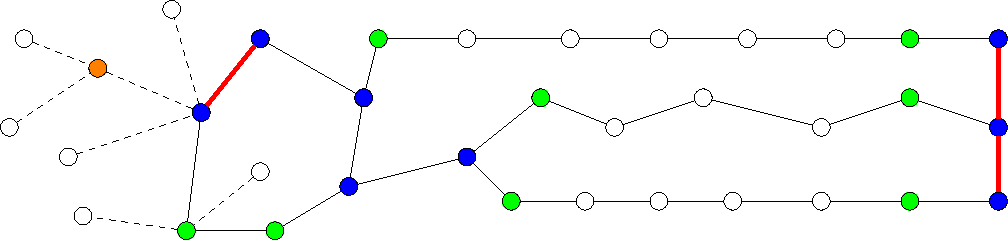
\includegraphics[width=0.8\columnwidth]{fig-example-names-vertices}
	\caption{An example of a graph with its important vertices: $U$ (in blue), $U^*$ (in green) and $Z^*$ (in orange).
    Corresponding feedback edges are marked with a thick red line, while dashed edges represent the edges (and vertices) ``removed'' from $G'$ at the initial step.
	\label{fig:labelingVertices}}
\end{figure}

% \medskip 
% \noindent We can solve \deltaExact\  by 
% for every pair of vertices $v_i, v_j \in V(G)$ we
% \begin{itemize}
%     \item determine the underlying path $P$ of the fastest temporal path from $v_i$ to $v_j$,
% for which we introduce the equality constraint (\ie $d(P) = D_{v_i, v_j}$), and %in the ILP
% \item make sure that every other path $P'$ from $v_i$ to $v_j$ is not faster than $P$ (\ie $d(P') \geq D_{v_i, v_j}$). %in the ILP
% \end{itemize}
% One could easily achieve this by ``guessing'' the fastest paths among each pair of vertices, but this would result in too many guesses. 
% With this in mind we create the following guesses.


\subparagraph{Guesses.} 
For every pair of important vertices $u,v \in U \cup U^{\ast} \cup Z^{\ast}$, we guess the sequence of edges in the fastest temporal path from $u$ to $v$. Since $U \cup U^{\ast} \cup Z^{\ast}\in O(k^2)$ and there are $k^{O(k)}$ possibilities for a sequence of edges between a fixed vertex pair, we have $k^{O(k^5)}$ overall possible guesses. We  defer further details to the Appendix (see guesses \textcolor{lipicsGray}{\textsf{\textbf{G-1}}} to \textcolor{lipicsGray}{\textsf{\textbf{G-6}}}).

\setcounter{guesscounter}{6}

\begin{figure}[t]
	\centering
	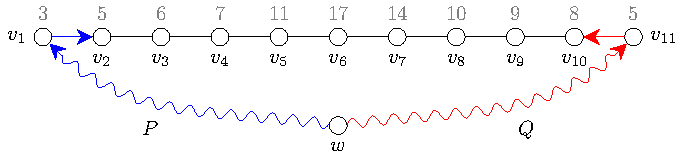
\includegraphics[width=0.75\columnwidth]{fig-exampleg10}
	\caption{In the above graph vertices $v_1, v_{11}, w$ are in $U$, while $v_2, v_{10}$ are in $U^*$. 
		Numbers above all $v_i$ represent the values of the fastest temporal paths from $w$ to each of them (\ie the entries in the $w$-th row of matrix $D$).
		From the basic guesses we know the fastest temporal path $P$ from $w$ to $v_2$ (depicted in blue) and the fastest temporal path $Q$ from $w$ to $v_{10}$.
		From the values of durations from $w$ to each $v_i$ we cannot 
		determine the fastest paths from $w$ to all $v_i$.
		More precisely, we know that $w$ reaches $v_2, v_3, v_4, v_5$ (resp.~$v_{10}, v_{9}, v_{9}, v_{7}$) 
		by first using the path $P$ (resp.~$Q$) and then proceeding through the vertices,
		but we do not know how $w$ reaches $v_6$ the fastest.
		Therefore we have to introduce some more guesses.
  \label{fig:guesses-advanced}}
\end{figure}

With the information provided by the described guesses we are still not able to determine all fastest paths. For example consider the case depicted in \cref{fig:guesses-advanced}. 
Therefore we introduce additional guesses that provide us with sufficient information to determine all fastest paths. To do this we have to first define the following.
\begin{definition}\label{def:segments}
	Let $U \subseteq V(G')$ be a set of vertices of interest and let $u,v \in U$.
	A path $P = (u=v_1,v_2, \dots, v_p = v)$  in graph $G'$, where all inner vertices are not in $U$, \ie $v_i \notin U$ for all $i \in \{ 2, 3, \dots, p-1\}$,
	is called a \emph{segment} from $u$ to $v$. We denote it as $S_{u,v}$.
\end{definition}
Note by \cref{def:segments} that $S_{u,v} \neq S_{v,u}$. 
Observe that a temporal path in $G'$ between two vertices of interest is either a segment, or it consists of a sequence of some segments. Furthermore, since we have at most $4k$ interesting vertices in $G'$, we can deduce the following important result.
\begin{corollary}\label{obs:FPT-k2segments}
	There are at most $O(k^2)$ segments in $G'$.
\end{corollary}
% We now continue with our guessing.
To describe the next guesses, we introduce the following notation. Let $u,v,x$ be three vertices in $G'$. We write $u \leadsto x \rightarrow v$ to denote a temporal path from $u$ to $v$ that passes through $x$, and then goes directly to $v$ (via one edge).
%In the case when we want to guess the fastest path from $u$, that passes through vertex $x$ (not necessarily via one edge), and then goes directly to $v$ (via one edge), we write it as a fastest path of the form $u \leadsto x \rightarrow v$.
We guess the following structures.
\begin{enumerate}[G-1.]
	\setcounter{enumi}{\value{guesscounter}}
	\item \label{FPT-guessFTPamongv2z2}
	\textbf{Inner segment guess I}.
	Let $S_{u,v} = (u=v_1,v_2, \dots, v_p = v)$ and $S_{w,z} = (w=z_1,z_2, \dots, z_r = z)$ be two segments. %,
	%first one between vertices $u,v \in U$, second one between vertices $w, z \in U$.
	We want to guess the fastest temporal path
	$v_2 \rightarrow u \leadsto w \rightarrow z_2$. 
	We repeat this procedure for all pairs of segments.
	Since there are $O(k^2)$ segments in $G'$,
	there are $k^{O(k^5)}$ possible paths of this form. \\
	Recall that $S_{u,v}\neq S_{v,u}$ for every $u,v\in U$. Furthermore note that we did not assume that $\{u,v\} \cap \{w,z\} = \emptyset$. Therefore, by repeatedly making the above guesses, we also guess the following fastest temporal paths: 
	${v_2 \rightarrow u \leadsto z \rightarrow z_{r-1}}$,\ \ \ 
	${v_2 \rightarrow u \leadsto v \rightarrow v_{p-1}}$,\ \ \  
	${v_{p-1} \rightarrow v \leadsto w \rightarrow z_{2}}$,\ \ \  
	${v_{p-1} \rightarrow v \leadsto z \rightarrow z_{r-1}}$, and  
	${v_{p-1} \rightarrow v \leadsto u \rightarrow v_{2}}$.
	%
	For an example see~\cref{fig:FPT-guessG4}.
	\item \label{FPT:guess-uToSegmentz2}
	\textbf{Inner segment guess II}.
	Let $S_{u,v} = (u=v_1,v_2, \dots, v_p = v)$ be a line segment in $G'$,
	and let $w \in U \cup Z^*$. %be either a vertex of interest or a representative vertex of a tree, whose clipped vertex is a vertex of interest.
	We want to
	guess the following fastest temporal paths
	$w \leadsto u \rightarrow v_2$, $w \leadsto v \rightarrow v_{p-1} \rightarrow \cdots \rightarrow v_2$,
	and
	$v_2 \rightarrow u \leadsto w$, $v_2 \rightarrow v_3 \rightarrow \cdots v \leadsto w$.
	\\
	For fixed $S_{u,v}$ and $w \in U \cup Z^*$ we have $k^{O(k)}$ different possible such paths, therefore we make $k^{O(k^4)}$ guesses for these paths.
	%
	For an example see~\cref{fig:FPT-guessG5}.
	%All together we made $O(k^{k^4}$  new guesses for the structure of all of the above mentioned fastest temporal paths.
	%Each of the previous partial ILP instances is therefore extended into $O(k^6)$ new ILP instances.
	\item \label{FPT:guess-splitFromAnotherSegmentAndPaths}
	\textbf{Split vertex guess I}.
	Let $S_{u,v} = (u=v_1,v_2, \dots, v_p = v)$ be a line segment in $G'$, and let us
	fix a vertex $v_i \in S_{u,v} \setminus \{u,v\}$.
	In the case when $S_{u,v}$ is of length $4$, the fixed vertex $v_i$ is the middle vertex, else we fix an arbitrary vertex $v_i \in S_{u,v} \setminus \{u,v\}$.
	Let 
	$S_{w,z} = (w=z_1,z_2, \dots, z_r = z)$ be another segment in $G'$.
	We want to determine the fastest paths from $v_i$ to all inner vertices of $S_{w,z}$. We do this by inspecting the values in matrix $D$ from $v_i$ to inner vertices of $S_{w,z}$.
	We split the analysis into two cases.
	\begin{enumerate}
		\item 
		There is a single vertex $z_j \in S_{w,z}$ for which the duration from $v_i$ is the biggest.
		More specifically, $z_j \in S_{w,z} \setminus \{w,z\}$ is the vertex with the biggest value  $D_{v_i,z_j}$.
		We call this vertex a \emph{split vertex of $v_i$ in the segment $S_{wz}$}.
		Then it holds that $D_{v_i,z_2} < D_{v_i,z_3} < \dots < D_{v_i,z_j}$ and 
		$D_{v_i,z_{r-1}} < D_{v_i,z_{r-2}} < \dots < D_{v_i,z_j}$.
		From this it follows that the fastest temporal paths from $v_i$ to $z_2, z_3, \dots, z_{j-1}$ go through $w$,
		and 
		the fastest temporal paths from $v_i$ to $z_{r-1}, z_{r-2}, \dots, z_{j+1}$ go through $z$.
		We now want to guess which vertex $w$ or $z$ is on a fastest temporal path from $v_i$ to $z_j$.
		Similarly,
		all fastest temporal paths starting at $v_i$ have to go either through $u$ or through $v$,
		which also gives us two extra guesses for the fastest temporal path from $v_i$ to $z_j$.
		Therefore, all together we have $4$ possibilities on how the fastest temporal path from $v_i$ to $z_j$ starts and ends.
		Besides that we want to guess also how the fastest temporal paths from $v_i$ to $z_{j-1}, z_{j+1}$ start and end.
		Note that one of these is the subpath of the fastest temporal path from $v_i$ to $z_j$, and the ending part is uniquely determined for both of them,
		\ie to reach $z_{j-1}$ the fastest temporal path travels through $w$, and to reach $z_{j+1}$ the fastest temporal path travels through $z$.
		Therefore we have to determine only how the path starts, namely if it travels through $u$ or $v$.
		This introduces two extra guesses.
		For a fixed $S_{u,v}, v_i$ and $S_{w,z}$ we find the vertex $z_j$ in polynomial time, 
		or determine that $z_j$ does not exist.
		We then make four guesses where we determine how the fastest temporal path from $v_i$ to $z_j$ passes through vertices $u,v$ and $w,z$ and 
		for each of them two extra guesses to determine the fastest temporal path from $v_i$ to $z_{j-1}$ and from $v_i$ to $z_{j+1}$.
		We repeat this procedure for all pairs of segments,
		which results in producing $k^{O(k^5)}$ new guesses.
		Note, $v_i \in S_{u,v}$ is fixed when calculating the split vertex for all other segments $S_{w,z}$.
		\item 
		There are two vertices $z_j, z_{j+1} \in S_{w,z}$ for which the duration from $v_i$ is the biggest.
		More specifically, $z_j, z_{j+1} \in S_{w,z} \setminus \{w,z\}$ are the vertices with the biggest value  $D_{v_i,z_j} = D_{v_i,z_{j+1}}$.
		Then it holds that $D_{v_i,z_2} < D_{v_i,z_3} < \dots < D_{v_i,z_j} = D_{v_i,z_{j+1}} > D_{v_i,z_{j + 2}} > \cdots > D_{v_i,z_{r-1}}$.
		From this it follows that the fastest temporal paths from $v_i$ to $z_2, z_3, \dots, z_{j}$ go through $w$,
		and 
		the fastest temporal paths from $v_i$ to $z_{r-1}, z_{r-2}, \dots, z_{j+1}$ go through $z$.
		In this case we only need to guess the following two fastest temporal paths 
		$u \leadsto w \rightarrow z_2$
		and $u \leadsto z \rightarrow z_{r-1}$.
		Each of this paths we then uniquely extend along the segment $S_{w,z}$ up to the vertex $v_j$, resp.~$v_{j+1}$,
		which give us fastest temporal paths from $u$ to $v_j$ and from $u$ to $v_{j+1}$.
		In this case we do not introduce any new guesses, as we have aready guessed 
		the fastest paths of the form
		$u \leadsto w \rightarrow z_2$
		and $u \leadsto z \rightarrow z_{r-1}$
		(see guess~\textcolor{lipicsGray}{\textsf{\textbf{G-\ref{FPT:guess-uToSegmentz2}}}}).
	\end{enumerate}
	Note that this case results also in knowing the fastest paths from the vertex $v_i \in S_{u,v}$ to $w,z \in S_{w,z}$ for all segments $S_{w,z}$, 
	\ie we know the fastest paths from a fixed $v_i \in S_{u,v}$ to all vertices of interest in $U$.
	%
	For an example see~\cref{fig:FPT-guessG6}.
	\item \label{FPT:guess-splitFromUtoAnotherSegment}
	\textbf{Split vertex guess II}.
	Let $w \in U \cup Z^*$ 
	and let $S_{u,v} = (u=v_1,v_2, \dots, v_p = v)$.
	We want to guess a split vertex of $w$ in $S_{u,v}$, and the fastest temporal path that reaches it.
	We again have two cases,
	first one where $v_i$ is a unique vertex in $S_{u,v}$ that is furthest away from $w$,
	and the
	second one where $v_i, v_{i+1}$ are two incident vertices in $S_{u,v}$, that are furthest away from $w$.
	\begin{comment}
	In first case we know exactly how the fastest paths from $w$ to all vertices $v_j \in S_{u,v} \setminus \{v_i\}$
	travel through the segment $S_{u,v}$ (\ie either through $u$ or $v$).
	Therefore we have to guess how the fastest path from $w$ reaches vertex $v_i$,
	we have two options, either it travels through $u \rightarrow v_2 \rightarrow \cdots \rightarrow v_{i-1} \rightarrow v_i$
	or 
	$v \rightarrow v_{p-1} \rightarrow \cdots \rightarrow v_{i+1} \rightarrow v_i$.
	Which produces two new guesses.
	In the second case we know exactly how the fastest temporal path reaches $v_i$ and $v_{i+1}$, and consequently all the inner vertices.
	Therefore no new guesses are needed.
	Note that the above guesses, together with the guesses from G-\ref{FPT:guess-uToSegmentz2},
	uniquely determine fastest temporal paths from $w$ to all vertices in $S_{u,v}$ 
	(this also holds for the case when $w \in S_{u,v}$, \ie $w = u$ or $w = v$).
	\end{comment}
	All together we make two guesses for each pair of vertex $w \in U$ and segment $S_{u,v}$.
	We repeat this for all vertices of interest, and all segments,
	which produces $k^{O(k^2)}$ new guesses.
	%
	For an example see~\cref{fig:FPT-guessG7}.
	Detailed analysis follows arguing from above (as in \textcolor{lipicsGray}{\textsf{\textbf{G-\ref{FPT:guess-splitFromAnotherSegmentAndPaths}}}}) and is deferred to Appendix.
	% counter for guesses continues
	\setcounter{guesscounter}{\value{enumi}}
\end{enumerate}
%
\begin{figure}[t]
	\centering
	\begin{subfigure}[b]{0.48\textwidth}
		\centering
		\resizebox{0.88\linewidth}{!}{
			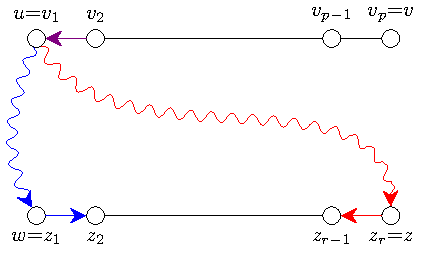
\includegraphics{fig-guess1}}
		\caption{Example of an Inner segment guess I (\textcolor{lipicsGray}{\textsf{\textbf{G-\ref{FPT-guessFTPamongv2z2}}}}), where we guessed the fastest temporal paths of the form $v_2 \rightarrow u \leadsto w \rightarrow z_2$ (in blue)
			and $v_2 \rightarrow u \leadsto z \rightarrow z_{r-1}$ (in red).
			\label{fig:FPT-guessG4}}
	\end{subfigure}
	\quad
	\begin{subfigure}[b]{0.48\textwidth}
		\centering
		\resizebox{0.88\linewidth}{!}{
			
			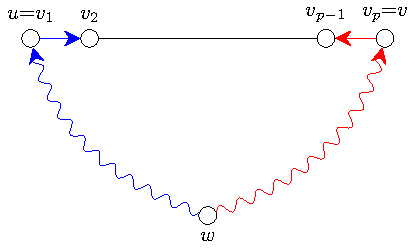
\includegraphics{fig-guess2}}
		\caption{Example of an Inner segment guess II (\textcolor{lipicsGray}{\textsf{\textbf{G-\ref{FPT:guess-uToSegmentz2}}}}), where we guessed the fastest temporal paths of the form $w \leadsto u \rightarrow v_2$ (in blue) and $w \leadsto v \rightarrow v_{p-1}$ (in red). 
			\label{fig:FPT-guessG5}}
	\end{subfigure}
	
	\begin{subfigure}[b]{0.48\textwidth}
		\vspace{-0.4cm}
        \centering
		\resizebox{0.98\linewidth}{!}{
			%
			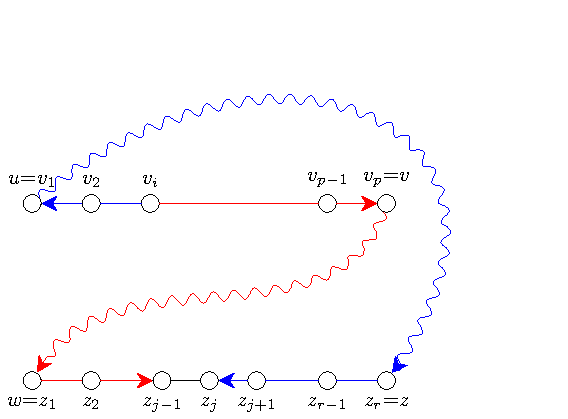
\includegraphics{fig-guess3}}
		\caption{Example of a Split vertex guess I (\textcolor{lipicsGray}{\textsf{\textbf{G-\ref{FPT:guess-splitFromAnotherSegmentAndPaths}}}}), where, for a fixed vertex $v_i \in S_{u,v}$,
			we calculated its corresponding split vertex $z_j \in S_{w,z}$,
			and guessed the fastest paths of the form
			$v_i \rightarrow v_{i-1} \rightarrow \cdots \rightarrow u \leadsto z \rightarrow z_{r-1} \cdots \rightarrow z_j$ (in blue) 
			and $v_i \rightarrow v_{i+1} \rightarrow \cdots \rightarrow v \leadsto w \rightarrow z_2 \rightarrow \cdots \rightarrow z_{j-1}$ (in red). 
			\label{fig:FPT-guessG6}}
	\end{subfigure}
	\quad
	\begin{subfigure}[b]{0.48\textwidth}
		\centering
		\resizebox{0.88\linewidth}{!}{
			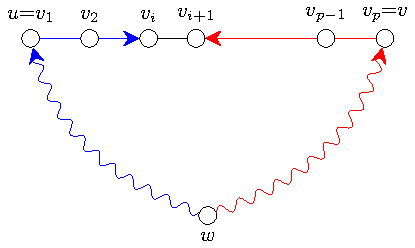
\includegraphics{fig-guess4}}
		\caption{Example of a Split vertex guess II (\textcolor{lipicsGray}{\textsf{\textbf{G-\ref{FPT:guess-splitFromUtoAnotherSegment}}}}), where, for a vertex of interest $w$, 
			we
			calculated its corresponding split vertex $v_i \in S_{u,v}$,
			and guessed the fastest paths of the form
			$w \leadsto u \rightarrow v_2 \rightarrow \cdots \rightarrow v_i$  (in blue) 
			and $w \leadsto v \rightarrow v_{p-1} \rightarrow \cdots \rightarrow v_{i+1}$ (in red). 
			\label{fig:FPT-guessG7}}
	\end{subfigure}
	\caption{Illustration of the guesses \textcolor{lipicsGray}{\textsf{\textbf{G-\ref{FPT-guessFTPamongv2z2}}}}, \textcolor{lipicsGray}{\textsf{\textbf{G-\ref{FPT:guess-uToSegmentz2}}}}, \textcolor{lipicsGray}{\textsf{\textbf{G-\ref{FPT:guess-splitFromAnotherSegmentAndPaths}}}}, and \textcolor{lipicsGray}{\textsf{\textbf{G-\ref{FPT:guess-splitFromUtoAnotherSegment}}}}.}
\end{figure}
%


There are two more guesses \textcolor{lipicsGray}{\textsf{\textbf{G-11}}} and \textcolor{lipicsGray}{\textsf{\textbf{G-12}}} that are deferred to the Appendix. 
We prove in the Appendix that, for all guesses \textcolor{lipicsGray}{\textsf{\textbf{G-1}}} to \textcolor{lipicsGray}{\textsf{\textbf{G-12}}}, there are in total at most $f(k)$ possible choices, and for each one of them we create an ILP with at most $f(k)$ variables and at most $f(k)\cdot |D|^{O(1)}$ constraints. Each of these ILPs can be solved in FPT time by Lenstra's Theorem~\cite{Lenstra1983Integer}.
%We create all of the above guesses independently.
%We start with the first one, that results in $O(k^{k^3})$ different possibilities, then we split each one of these guesses into $O(k^{k^3})$ new ones, that respond to the guessing in the second step, etc.
%After creating all of the guesses we end up with $f(k)$ different cases (where $f$ is a double exponential) 
%and create one ILP instance for each case.
%
%For each of the ILP instances we iterate through all pairs of vertices $u,v \in V(G)$ and, using the above guesses, determine, not only the fastest path $P$ from $u$ to $v$, but also all other paths $P'_i$.
%For the labels of edges of the fastest path $P$ we introduce the equality constraint, while for the labels of the edges of all other paths $P'_i$ we introduce the inequality constraint (\ie the duration $d(P_i')$ of any $P'_i$ cannot be smaller than $d(P)=D_{u,v}$).
%We can do this efficiently, while introducing only a small number of variables,
%which ensures that each ILP is solved in an FPT-time.
For detailed explanation and proofs of this part see Appendix.


\section{Conclusion}\label{sec:conclusion}
We believe that our work spawns several interesting future research directions and builds a base upon which further temporal graph realization problems can be investigated.

%\subparagraph{Further parameterizations.} 
There are several structural parameters which can be considered to obtain tractability which are either larger or incomparable to the feedback vertex number. We believe that the \emph{vertex cover number} or the \emph{tree depth} are promising candidates.
Furthermore, we can consider combining a structural parameter such as the \emph{treewidth} with $\Delta$.

%\subparagraph{Further problem variants.}
There are many natural variants of our problem that are well-motivated and warrant consideration. 
%In the following, we give two specific examples. 
We believe that one of the most natural generalizations of our problem is to allow more than one label per edge in every $\Delta$-period. A well-motivated variant (especially from the network design perspective) of our problem would be to consider the entries of the duration matrix $D$ as upper-bounds on the duration of fastest paths rather than exact durations. 
Our work gives a starting point for many interesting future research directions such as the two mentioned examples.



\bibliography{bibliography}	


%\clearpage

%\appendix


\end{document}